% created on 2019-12-13
% @author : bmazoyer

%% Lines to compile only this capter
\documentclass[11pt, twoside, a4paper, openright]{report}
\usepackage[utf8]{inputenc}
% \DeclareUnicodeCharacter{223C}{~}

%Bibliography style
% \usepackage[square, numbers]{natbib}
% \usepackage[round]{natbib}
% \usepackage{biblatex}
% \bibliographystyle{unsrtnat}
% \bibliographystyle{unsrt}
% \bibliographystyle{plain}
% \bibliographystyle{aa}
% \usepackage[backend=bibtex,style=authoryear,natbib=true]{biblatex} 
\usepackage[
backend=biber,
style=authoryear,
citestyle=authoryear,
url=false
]{biblatex}
\addbibresource{../source/library.bib}

\usepackage[T1]{fontenc}
\usepackage[french]{babel}
\usepackage{csquotes}  % used for citations (recommended when using biblatex)
%\usepackage{helvet}
%\renewcommand{\familydefault}{\sfdefault}
\usepackage{mathptmx}
\usepackage{amssymb}
\usepackage{geometry} 
\usepackage{xcolor}
\usepackage[absolute,overlay]{textpos}
\usepackage{graphicx}
\usepackage{lipsum}
\usepackage[explicit]{titlesec}
\usepackage{lmodern}
\usepackage{color}
\usepackage{array}
\usepackage{mathtools}
\usepackage{caption}
\usepackage{multicol}
\usepackage{booktabs}
\usepackage{enumitem}
\usepackage{hyperref}
\usepackage{afterpage}
\usepackage{emptypage}
\usepackage{setspace}
\usepackage{pgffor}
    \setlength{\columnseprule}{0pt}
    \setlength\columnsep{10pt}
\usepackage[francais,nohints]{minitoc}
    \setcounter{minitocdepth}{3}
 
 %https://la-bibliotex.fr/2019/02/03/ecrire-les-nombres-et-les-unites-avec-latex/   
\usepackage{siunitx}
% \sisetup{
%     detect-all,
%      output-decimal-marker={,},
%      group-minimum-digits = 3,
%      group-separator={~},
%      number-unit-separator={~},
%      inter-unit-product={~},
%      list-separator = {, },
%      list-final-separator = { et },
%      range-phrase = --,
%      separate-uncertainty = true,
%      multi-part-units = single,
%      list-units = single,
%      range-units = single
%     }
\usepackage{physics}
\usepackage{isotope}

\usepackage[perpage]{footmisc} % to reset the counter of footnote each page

    
\usepackage{fancyhdr}			% Entête et pieds de page. Doit être placé APRES geometry
\pagestyle{fancy}		% Indique que le style de la page sera justement fancy
%\lfoot[\thepage]{} 		% gauche du pied de page
%\cfoot{} 			% milieu du pied de page
%\rfoot[]{\thepage} 
\fancyfoot{} % vide le pied~de~page
\fancyfoot[LE,RO]{\thepage}
\fancyfoot[LO,CE]{}% droite du pied de page
\fancyhead{}	
\fancyhead[LE]{\leftmark}	
\fancyhead[RO]{\rightmark}

\fancypagestyle{plain}{%
\fancyhf{} % vide l’en-tête et le pied~de~page.
\fancyfoot[LE,RO]{\thepage} % numéro de la page en cours en gras% et centré en pied~de~page.
\renewcommand{\headrulewidth}{0pt}
\renewcommand{\footrulewidth}{0pt}}



% Premiere page des chapitres
\newlength\chapnumb
\setlength\chapnumb{3cm}
 
\titleformat{\chapter}[block] {
  \normalfont}{}{0pt} { %police
    \parbox[b]{\chapnumb}{
      \fontsize{120}{110}\selectfont\thechapter} %taille du chiffre
      \parbox[b]{\dimexpr\textwidth-\chapnumb\relax}{
        \raggedleft 
        \hfill{\bfseries\Huge#1}\\ %taille du titre
        \rule{\dimexpr\textwidth-\chapnumb\relax}{0.4pt} %ligne de separation
  }
}
 
 %premiere page chapitre non numerote (remerciement, table des matieres ...)
 
\titleformat{name=\chapter,numberless}[block]
{\normalfont}{}{0pt}
{   
    \parbox[b]{\dimexpr\textwidth}{%   
    \hfill{\bfseries\Huge#1}\\
  \rule{\dimexpr\textwidth}{0.4pt}}}
    
 %   \titleformat{name=\chapter,numberless}[block]
%{\normalfont}{}{0pt}
%{\parbox[b]{\chapnumb}{%
%   \mbox{}}%
%  \parbox[b]{\dimexpr\textwidth-\chapnumb\relax}{%
%    \raggedleft%
%    \hfill{\bfseries\Huge#1}\\
%    \rule{\dimexpr\textwidth-\chapnumb\relax}{0.4pt}}}


%%%    SIunitx
\sisetup{locale = FR,
  % inter-unit-product=\ensuremath{\cdot},
  inter-unit-product=\ensuremath{\,},
  per-mode=reciprocal,
  separate-uncertainty = true,
  detect-all
}
\DeclareSIUnit{\Mpc}{Mpc}
\DeclareSIUnit{\kpc}{kpc}
\DeclareSIUnit{\Gpc}{Gpc}
\DeclareSIUnit{\h}{\textit{h}~}
\DeclareSIUnit{\perh}{\textit{h}^{-1}\,}

%%% Geometry
\geometry{
left=20mm,
top=30mm,
right=20mm,
bottom=30mm
}

%%% Color
\definecolor{bordeau}{rgb}{0.3515625,0,0.234375}

%%% Commands
\newcommand{\Nmocks}{\num{30}}
\newcommand{\hMpc}{h^{-1}\,\mathrm{Mpc}}
\newcommand{\hGpc}{h^{-1}\,\mathrm{Gpc}}
\newcommand{\kms}{\mathrm{km\,s^{-1}}}

\newcommand{\lya}{Ly$\alpha$}
\newcommand{\lyb}{Ly$\beta$}
\newcommand{\lyalya}{Ly$\alpha$(Ly$\alpha$)}
\newcommand{\lyalyb}{Ly$\alpha$(Ly$\beta$)}

\newcommand{\lrf}{\lambda_{\rm RF}}
\newcommand{\kpar}{k_{\parallel}}
\newcommand{\apar}{\alpha_{\parallel}}
\newcommand{\rpar}{r_{\parallel}}
\newcommand{\aperp}{\alpha_{\perp}}
\newcommand{\rperp}{r_{\perp}}
\newcommand{\kperp}{k_{\perp}}

\newcommand{\blya}{b_{\rm Ly\alpha}}
\newcommand{\betalya}{\beta_{\rm Ly\alpha}}
\newcommand{\blyb}{b_{\rm Ly\alpha}}
\newcommand{\betalyb}{\beta_{\rm Ly\beta}}
\newcommand{\dlya}{d_{\rm Ly\alpha}}
\newcommand{\bhcd}{b_{\rm HCD}}
\newcommand{\betahcd}{\beta_{\rm HCD}}
\newcommand{\Fhcd}{F_{\rm HCD}}
\newcommand{\Lhcd}{L_{\rm HCD}}

\newcommand{\imin}{i_{\rm min}}
\newcommand{\imax}{i_{\rm max}}
\newcommand{\jmin}{j_{\rm min}}
\newcommand{\jmax}{j_{\rm max}}

\newcommand{\xioned}{\xi_{\rm 1d}}
\newcommand{\DHub}{D_{H}}
\newcommand{\DM}{D_{M}}

\newcommand{\omegam}{\Omega_M}
\newcommand{\omegac}{\Omega_C}
\newcommand{\omegab}{\Omega_B}
\newcommand{\omegan}{\Omega_\nu}
\newcommand{\omegal}{\Omega_\Lambda}
\newcommand{\omegak}{\Omega_k}
\newcommand{\orad}{\Omega_R}
\newcommand{\ogam}{\Omega_\gamma}
\newcommand{\lcdm}{$\Lambda$CDM}

\newcommand{\picca}{\texttt{picca}}

%%% Rem's command
\newcommand\blankpage{%
    \null
    \thispagestyle{empty}%
    \addtocounter{page}{-1}%
    \newpage}
  
% Command to set up a particular alignment for a cell in tabular :
% \myalign{c}{foo} for instance
\newcommand*{\myalign}[2]{\multicolumn{1}{#1}{#2}}
 
\renewcommand{\thesection}{\arabic{section}}

% Romain
\newcommand{\cRM}[1]{\MakeUppercase{\romannumeral #1}}	% Capital
\newcommand{\cRm}[1]{\textsc{\romannumeral #1}}	% Petit majuscule
\newcommand{\crm}[1]{\romannumeral #1}
% Siècle %
\newcommand{\siecle}[1]{\cRm{#1}\textsuperscript{e}~siècle}



% Thesis title
\newcommand{\PhDTitle}{Les forêts \lya{} du relevé eBOSS : comprendre les fonctions de corrélation et les systématiques} 

% Name
\newcommand{\PhDname}{Thomas Etourneau} 

% Change this variable if you add or remove chapters
\newcommand*{\NumOfChapters}{6}

% Change this variable if you add or remove appendices
\newcommand*{\NumOfAppendices}{2}

% PDF metadata
\hypersetup{
	pdfauthor={\PhDname},
	pdfsubject={Manuscrit de thèse de doctorat},
	pdftitle={\PhDTitle}
}


\begin{document}
%%

\graphicspath{ {../figures/mocks_ana/} }

\chapter{Validation des mocks}
\minitoc
\newpage
\thispagestyle{fancy}


\textbf{Ce chapitre a pour vocation de présenter l'analyse menée sur les mocks, afin de valider leur construction et le choix des différents paramètres.
Nous présentons d'abord les estimateurs des diverses fonctions de corrélations, puis les modèles ajustés sur celles-ci.
Nous donnons premièrement le modèle ajusté sur les données et présenté dans \textcite{prov}, puis le modèle modifié ajusté sur les mocks.
Enfin, nous présentons l'analyse des \Nmocks{} réalisations de mocks produites. Le résultat de l'analyse des données, utilisée pour choisir les paramètres \lya{} des mocks, est présentée dans le chapitre suivant.
Toutes ces analyses sont produites avec le code \texttt{picca}. Ce code permet de calculer les champs $\delta$, les fonctions de corrélations, les matrices de distorsion, les matrices de covariance ainsi que de réaliser l'ajustement du modèle.}

\section{Les estimateurs}
Nous présentons ici les estimateurs utilisés pour calculer la fonction d'auto-corrélation du \lya{}, la fonction de corrélation croisée \lya{}-QSO, ainsi que la fonction d'auto-corrélation d'objets ponctuels tels les quasars.
% Dans le cas des objets ponctuels, la seule information nécessaire au calcul de la fonction de corrélation est le catalogue fournissant pour chaque objet l'ascension droite, la déclinaison et le redshift.
\textbf{
  Dans le cas des objets ponctuels, il est nécessaire de produire un catalogue aléatoire d'objets qui prend en compte la complétude\footnote{La complétude donne la proportion de cibles observées en spectroscopie par rapport au nombre de cibles détectées avec le relevé photométrique.} du relevé spectrométrique. %, ainsi que les effets liés à la sélection des cibles afin de calculer correctement la fonction d'auto-corrélation. % Un tel catalogue est produit pour chaque réalisation des mocks.
  Il est aussi nécessaire d'estimer l'inhomogénéité de la sélection des cibles, afin de pondéré chaque quasar par un poids qui vise à la corriger.
}
% Pour le calcul des fonctions de corrélation impliquant le \lya{}, il est nécessaire de calculer au préalable le champ $\delta_F$ (équation~\ref{eq:deltaF}).
\textbf{Pour le calcul des fonctions de corrélation impliquant le \lya{}, il n'est pas utile d'avoir un catalogue aléatoire. En effet, le champ $\delta_F$ nous donne directement accès, à un biais près, au contraste de densité. Nous pouvons donc calculer la fonction de corrélation avec une formule du type de l'équation~\ref{eq:def_cf}, ce qui n'est pas possible dans le cas des objets ponctuels, et nous n'avons pas besoin de tenir compte de l'homogénéité de la sélection des cibles. Les poids servent donc uniquement à maximiser le rapport signal sur bruit.
  % Ceci nous permet aussi de ne pas tenir compte de l'homogénéité de la sélection des cibles, et donc d'utiliser des poids qui servent uniquement à maximiser le rapport signal sur bruit.}
  }

Pour le calcul du champ $\delta_F$, nous distingons deux cas : le cas où nous analysons les \emph{raw mocks} et le cas où nous analysons les \emph{cooked mock} ou les données.
Les raw mocks (les mocks bruts, non préparés) désignent les mocks avant d'avoir tourné le code \texttt{quickquasars}.
Les fonctions de corrélation sont alors calculées en utilisant directement la fraction de flux transmise $F$ donnée dans les fichiers de transmissions. Etant donné que pour chaque forêt, nous avons directement accès à $F$, le champ $\delta_F$ est donné par
\begin{equation}
  \delta_F = \frac{F}{\overline F(z)} - 1 \; .
\end{equation}
Les cooked mocks quant à eux désignent les mocks après avoir appliqué \texttt{quickquasars} à chaque forêt. Dans ce cas, comme pour les données, la fraction de flux transmise $F$ n'est pas accessible. Il faut alors utiliser la procédure d'ajustement du continuum décrite dans la section~\ref{subsec:calcul_delta}.
Une fois le champ $\delta_F$ calculé, nous pouvons calculer les différentes fonctions de corrélation.

\subsection{L'auto-corrélation \lya{}$\times$\lya{}}
Comme expliqué dans le chapitre d'introduction, la fonction d'auto-corrélation du champ d'absorption $F$ du \lya{} est définie comme
\begin{equation}
  \xi_{\mathrm{Ly}\alpha}(\vec r) = \langle \delta_F(\vec{r'}) \delta_F(\vec{r} + \vec{r'}) \rangle \; .
\end{equation}
% Elle peut-être mise sous la forme
Nous pouvons utiliser comme estimateur
\begin{equation}
 \hat \xi(\vec r) = \langle \delta_i \delta_j \rangle \; ,
\end{equation}
où $\langle .\rangle$ désigne la moyenne sur tous les pixels $i$ et $j$ qui vérifient $\vec r_{ij} = \vec r$.
Afin d'estimer $\xi_{\mathrm{Ly}\alpha}$, une grille en $(\rpar{}, \rperp{})$ est créée.
% Chaque bin de cette grille fait $(\SI{4}{\perh\Mpc})^3$.
Les bins mesurent \SI{4}{\perh\Mpc} dans chaque direction.
% Cette taille de bin permet à la fois de regrouper suffisamment de pixels pour avoir une bonne statistique dans chaque bin, mais aussi d'avoir suffisamment de bins pour résoudre correctement la région du pic BAO (\#prov est-ce que c'est vrai ? toujours la meme quantite d'info, donc ca ameliore pas le fit?).
Cette taille de bin est choisie de façon à avoir suffisamment de bins pour résoudre correctement la région du pic BAO, mais aussi de façon à ne pas avoir trop de bins pour le calcul de la matrice de covariance. La taille de bin choisie et la gamme en $r$ utilisée produisent déjà une matrice de covariance de \num{2500}$\times$\num{2500} bins.
% Une fois cette grille construite, nous transformons les coordonnées $(\alpha, \delta, z)$ des pixels $\delta_F$ en distances.
Une fois cette grille construite, la séparation de chaque paires $(\Delta \theta, \Delta z)$ est transformée en distance comobile afin d'obtenir la séparation $(\rpar{}, \rperp{})$ :
\begin{equation}
  \left\{
    \begin{array}{l}
      \rpar{} = \left[D_C(z_i) - D_C(z_j)\right] \cos\left(\frac{\Delta \theta}{2}\right) \; , \\
      \rperp{} = \left[D_M(z_i) - D_M(z_j)\right] \sin\left(\frac{\Delta \theta}{2}\right) \; ,
    \end{array}
  \right. 
\end{equation}
où $D_C$ est la distance comobile le long de la ligne de visée, et $D_M$ la distance comobile transverse (voir section~\ref{subsec:descri_mod}, paragraphe \emph{Les distances}). $z_i$ et $z_j$ sont les redshifts des pixels $i$ et $j$.
Puis, pour chaque bin $A$ de la grille en $(\rpar{}, \rperp{})$, toutes les paires de pixels dont la distance de séparation se trouve dans ce bin $A$ sont considérées. La fonction de corrélation dans ce bin est alors donnée par
\begin{equation}
  \label{eq:xiff}
  \xi_A = \frac{
    \sum\limits_{(i,j)\in A} w_i w_j \delta_i \delta_j
  }{
    \sum\limits_{(i,j)\in A} w_i w_j
  }
  \; ,
\end{equation}
% où $w_i$ est le poids associé au pixel $i$. Les poids utilisés dans le calcul des fonctions de corrélation sont les poids définis dans l'équation~\ref{eq:weights}, corrigés par la dépendance en redshift du champ d'absorption du \lya{}. Le champ du \lya{} varie comme
% \begin{equation}
%   \delta_{\mathrm{Ly}\alpha}(z) = \delta_{\mathrm{Ly}\alpha}(0) \frac{b_{\mathrm{Ly}\alpha}(z) G(z)}{b_{\mathrm{Ly}\alpha}(0)G(0)} \; .
% \end{equation}
% Le facteur de croissance varie comme $G(z) \propto (1+z)^{-1}$, et le biais du \lya{} comme $b_{\mathrm{Ly}\alpha}(z) \propto (1+z)^{\gamma}$.
% Le champ $\delta_{\mathrm{Ly}\alpha}(z)$ est donc proportionnel à $(1+z)^{\gamma - 1}$. Le paramètre $\gamma = 2.9$ est mesuré sur le spectre de puissance à une dimension du \lya \autocite{McDonald2004} (\#prov j'ai pas trouvé dans le papier à quel endroit était donnée la mesure).
% Ainsi, les poids utilisés dans l'équation~\ref{eq:xiff} sont donnés par
% \begin{equation}
%   \label{eq:weights2}
%   w_i = (1+z)^{\gamma - 1} \hat w_i \; ,
% \end{equation}
% où $\hat w_i$ sont les poids définis dans l'équation~\ref{eq:weights}.
% Le calcul de la fonction de corrélation est donc effectué à l'aide d'une double boucle sur les pixels.
où $w_i$ est le poids associé au pixel $i$. Ces poids sont définis dans l'équation~\ref{eq:weights2}. La correction de la dépendance en redshift du biais du \lya{} permet de donner plus de poids aux pixels à grand redshift, où l'amplitude de la fonction de corrélation est plus importante.
Le calcul de la fonction de corrélation est donc effectué à l'aide d'une double boucle sur les pixels.
Afin de réduire le temps de calcul, la fonction de corrélation est calculée uniquement pour les paires de pixels pour lesquelles $\rpar{}$ et $\rperp{}$ sont inclus dans $[0 \, ; 200] \si{\perh\Mpc}$. La fonction de corrélation est donc calculée dans $50 \times 50 = \num{2500}$ bins.
Les paires formées par des pixels provenant de la même forêt sont exclues du calcul afin d'éviter que les erreurs sur l'ajustement du continuum biaisent la mesure de la fonction de corrélation.

L'analyse \lya{} des données complète d'eBOSS \autocite{prov} utilise deux fonctions de corrélation distinctes : les fonctions de corrélation \lyalya{}$\times$\lyalya{} et \lyalya{}$\times$\lyalyb{}.
La région \lyb{} ne fournit pas suffisamment de pixels pour pouvoir calculer la fonction de corrélation \lyalyb{}$\times$\lyalyb{} et y détecter le pic BAO. De plus, le gain de statistique que représente cette fonction de corrélation est négligeable.
L'utilisation de ces deux fonctions de corrélation permet de mesurer la position du pic BAO avec une plus grande précision. Dans ce manuscrit, nous nous intéressons à la mesure de $b_{\mathrm{Ly}\alpha}$ et $\beta_{\mathrm{Ly}\alpha}$ afin de construire correctement nos mocks. Pour limiter les potentielles systématiques, nous considérons donc uniquement la fonction de corrélation \lyalya{}$\times$\lyalya{}.
Le graphique de droite de la figure~\ref{fig:pixel_number} présente les distributions pondérées en redshift des paires \lyalya{}$\times$\lyalya{} et \lyalya{}$\times$\lyalyb{}. L'analyse des données DR16 présentée dans ce manuscrit considère donc uniquement la distribution indiquée en orange.


\subsection{La corrélation croisée \lya{}$\times$QSO}
Nous donnons dans cette section l'estimateur de la fonction de corrélation croisée \lya{}$\times$QSO. De la même manière que précédemment, le calcul s'effectue dans des bins en $(\rpar{}, \rperp{})$. L'estimateur de la fonction de corrélation dans le bin $A$ est donnée par
\begin{equation}
  \label{eq:xiqf}
\hat  \xi_A = \frac{
    \sum\limits_{(i,j)\in A} w_i w_j \delta_i
  }{
    \sum\limits_{(i,j)\in A} w_i w_j
  }
  \; ,
\end{equation}
où l'indice $i$ court sur les pixels des forêts et $j$ sur les quasars pour lesquels la distance de séparation est comprise dans le bin $A$. Les paires $ij$ où le pixel $i$ appartient à la forêt du quasar $j$ sont rejetées.
% Aussi, comme pour le \lya{}, les poids $w_j$ associés aux quasars incluent la dépendance avec le redshift du biais des quasars. Similairement à l'équation~\ref{eq:weights2}, ils sont définis comme
Similairement au \lya{}, les poids $w_j$ associés aux quasars favorisent les quasars à plus grand redshift. Ces poids sont définis comme
\begin{equation}
  \label{eq:weights3}
  w_j = \left(\frac{1 + z_j}{1 + \num{2.25}}\right)^{\gamma_{\textsc{QSO}}} \; ,
\end{equation}
où $\gamma_{\textsc{QSO}} = \num{1.44} \pm \num{0.08}$ \autocite{Bourboux2019}. Dans le calcul de la fonction de corrélation croisée \lya{}$\times$QSO, nous nous restreignons aux paires pour lesquelles $\rperp{} \in [0 \, ; 200] \si{\perh\Mpc}$.
Contrairement à l'auto-corrélation du \lya{}, la fonction de corrélation croisée n'est pas symétrique en $\rpar{}$.
Cette assymétrie est produite par l'erreur systématique sur la mesure du redshift des quasars, et aussi par le rayonnement des quasars qui n'est pas isotrope.
La fonction de corrélation croisée est donc calculée dans les bins pour lesquels $\rpar{} \in [-200 \, ; 200] \si{\perh\Mpc}$. Ceci représente $100 \times 50 = \num{5000}$ bins.



\subsection{Le spectre de puissance à une dimension}
Comme expliqué dans le chapitre précédent, nous ajustons le spectre de puissance $P_{s}$ appliqué à $\delta_s$ de façon à obtenir un spectre de puissance à une dimension $P^{\mathrm{1D}}$ en accord avec les données. Nous présentons donc maintenant la mesure de ce spectre de puissance sur les raw mocks. Pour chaque forêt, nous appliquons une transformation de Fourier au champ $\delta_F$ afin d'obtenir le champ $\delta_k$. Puis, le spectre de puissance de cette forêt est obtenu comme
\begin{equation}
\hat  P^{\mathrm{1D}}(k) = \langle \delta_k^2 \rangle \; .
\end{equation}
Nous répétons cette procédure pour toutes les forêts, puis le spectre de puissance total est obtenu comme la moyenne du spectre de puissance de chaque forêt.

En ce qui concerne les données et les cooked mocks, la mesure du spectre de puissance à une dimension est plus complexe. Un certain nombre d'effets liés à la mesure doivent être pris en compte. En particulier, le bruit et la résolution doivent être estimés et pris en compte pour ne pas fausser l'estimation du spectre de puissance. Cette analyse est détaillée dans~\textcite{Chabanier2018}.

\subsection{La fonction de corrélation à une dimension}
  Nous présentons maintenant l'estimateur de la fonction de corrélation à une dimension. Similairement au $P^{\mathrm{1D}}$, cette fonction de corrélation est calculée en considérant uniquement les paires de pixels appartenant à la même forêt.
  Nous l'estimons comme
  \begin{equation}
\hat    \xi^{\mathrm{1D}}_A  = \frac{
      \sum\limits_{(i,j)\in A} w_i w_j \delta_i \delta_j
    }{
      \sum\limits_{(i,j)\in A} w_i w_j
    }
    \; ,
  \end{equation}
  où $w_i$ est le poids associé au pixel $i$. Ces poids sont définis dans l'équation~\ref{eq:weights2}
  % La fonction de corrélation à une dimension $\xi^{\mathrm{1D}}$ permet de mettre en avant les autres absorbeurs présents dans le champ d'absorption utilisé pour calculer le champ $\delta_F$. Ces absorbeurs produisent des pics dans la fonction de corrélation à une dimension. Ces pics sont aussi visibles dans les bins le long de la ligne de visée de la fonction de corrélation à trois dimensions (voir l'explication de la matrice des métaux, section~\ref{subsec:model_donnees}).
%  Elle est très affectée par les distorsions dues à l'ajustement du continu \#prov
  La fonction de corrélation à une dimension $\xi^{\mathrm{1D}}$ correspond à la fonction de corrélation à trois dimensions pour $\mu = 1$. En considérant uniquement les paires le long de la ligne de visée, elle permet de mettre en évidence les autres absorbeurs présents dans le milieu intergalactique, tels les métaux. La longueur d'onde d'absorption au repos de ces espèces étant différente de celle du \lya{}, les séparations physiques $\rpar{}=0$ sont reconstruite à une séparation $\rpar{}$ non nulle (voir l'explication de la matrice des métaux, section~\ref{subsec:model_donnees}). Ceci produit des pics dans la fonction de corrélation à une dimension. Ces pics sont d'autant plus visibles quand la fonction de corrélation est représentée en fonction de $\lambda_i / \lambda_j$, où $\lambda_i$ et $\lambda_j$ sont les longueurs des deux pixels formant chaque paire.
  % En effet, la séparation reconstruire $\rpar{}$ est donnée par
%   \begin{equation}
%     \rpar_{1,2}(\lambda_{\mathrm{obs}}) =  D_{C}(z = \frac{\lambda_{\mathrm{obs}}}{\lambda_1} - 1) - D_{C}(z = \frac{\lambda_{\mathrm{obs}}}{\lambda_2} - 1) \; ,
%   \end{equation}
% où $\lambda_{\mathrm{obs}}$ est la longueur d'onde observée, et $\lambda_1$ et $\lambda_2$ sont les longueurs d'ondes d'absorption au repos de l'absorbant 1 et 2.


\subsection{L'auto-corrélation QSO$\times$QSO}
Afin de tester les mocks sous tous leurs aspects, nous mesurons aussi l'auto-corrélation QSO$\times$QSO. L'estimateur utilisé pour cette corrélation est l'estimateur de Landy-Szalay \autocite{Landy1993}. C'est l'estimateur qui minimise la variance. Il est défini comme
\begin{equation}
  \label{eq:estimateur_co}
  \hat \xi = \frac{DD - 2DR + RR}{RR} \; .
\end{equation}
Les termes $DD$, $RR$ et $DR$ donnent les nombres de paires normalisés dans chaque bin ($\rpar{}$, $\rperp{}$). Ils sont donnés par
\begin{align}
  DD(\rpar{}, \rperp{}) &= \frac{dd(\rpar{}, \rperp{})}{n_d(n_d-1)/2} \; ,\\
  RR(\rpar{}, \rperp{}) &= \frac{rr(\rpar{}, \rperp{})}{n_r(n_r-1)/2} \; ,\\
  DD(\rpar{}, \rperp{}) &= \frac{dr(\rpar{}, \rperp{})}{n_dn_r}  \; ,
\end{align}
où $dd$ donne le nombre de paires mesuré dans les données, $rr$ le nombre de paires mesuré dans le catalogue aléatoire, et $dr$ le nombre de paires constituées d'un objet présent dans les données et d'un objet présent dans le catalogue aléatoire. $n_d$ et $n_r$ donnent respectivement le nombre d'objet constituant le catalogue des données et le catalogue aléatoire.
Nous utilisons aussi cet estimateur pour calculer la fonction d'auto-corrélation HCD$\times$HCD.


\section{Les matrices de distorsion}
\label{sec:calcul_dmat}
L'ajustement du continuum nécessaire au calcul du champ $\delta_F$ dans les données et les coocked mocks biaise le champ mesuré. Cependant, grâce à la transformation (équation~\ref{eq:deltaF3}) décrite dans la section~\ref{subsec:projdelta}), l'effet sur la fonction de corrélation peut-être pris en compte.
% L'idée est la suivante : plutôt que d'essayer de corriger la distorsion induite par l'ajustement du continuum sur la fonction de corrélation, cette distorsion est calculée et appliquée au modèle qui est ajusté aux données (\#prov pourquoi on inverse pas la dmat?).
L'idée est la suivante : modéliser la distorsion induite par l'ajustement du continuum et par la transformation~\ref{eq:deltaF3} sur la fonction de corrélation, appliquer cette distorsion au modèle, puis ajuster le modèle ``distordu'' aux données.
% L'ajustement du continuum et la transformation~\ref{eq:deltaF3} induisent des corrélations le long de la ligne de visée. 
L'effet le plus important de l'ajustement du continuum et de la transformation~\ref{eq:deltaF3} est de forcer la moyenne et la pente de chaque région spectrale à être nulle. Ceci induit des corrélations entre les pixels d'une même région spectrale, et donc le long de la ligne de visée.
Ainsi, au premier ordre, nous pouvons considérer que chaque $\delta_F$ après distorsion d'une forêt est une combinaison linéaire de tous les $\delta_F$ avant distorsion de cette forêt.
La fonction de corrélation distordue dans le bin $A$ peut alors être reliée à la vraie fonction de corrélation comme
\begin{equation}
  \xi_{\mathrm{distorsion}}(A) = \sum_{B} D_{AB}\xi_{vraie}(B) \; , 
\end{equation}
où $D_{AB}$ est appelée la \emph{matrice de distorsion}. Celle-ci s'exprime en fonction du terme $\eta_{ij}^q$, défini dans l'équation~\ref{eq:proj1}. Pour l'auto-corrélation, elle s'exprime comme
\begin{equation}
  \label{eq:dmat}
  D_{AB} = \frac{1}{W_A} \sum_{(i,j)\in A} w_i w_j \left( \sum_{(i',j')\in B} \eta_{ii'} \eta_{jj'} \right) \,
\end{equation}
où $W_{A} = \sum_{(i,j)\in A} w_i w_j$ est le poids du bin A. Pour la corrélation croisée, la matrice de distorsion est donnée par
\begin{equation}
  \label{eq:xdmat}
  D_{AB} = \frac{1}{W_A} \sum_{(i,j)\in A} w_i w_j \left( \sum_{(i',j')\in B} \eta_{ii'} \right) \, .
\end{equation}
Comme précédemment, les indices $i$ correspondent aux pixels des forêts, et $j$ aux quasars. A cause de la double somme, le calcul de la matrice de distorsion est très long. Afin de rendre possible l'estimation de cette dernière, le calcul est fait sur \SI{1}{\percent} des paires, tirées au hasard (\#prov Bautista 2017 montre que c'est OK avec 5\%, est-ce que y a une etude qui montre que c'est ok avec 1\% ? Dans DR14, ils utilisent 5\% je pense).
% L'étude présentée dans~\textcite{bautista_measurement_2017}

La figure~\ref{prov} (\#prov faire la figure) montre l'effet de la distorsion sur l'auto-corrélation \lya{}$\times$\lya{} dans les mocks. La fonction de corrélation est présentée dans quatres gammes en $\mu$. La courbe noire indique la fonction de corrélation calculée sur les raw mocks, et la courbe bleu la fonction de ....
\#prov Refaire la figure 11 de Bautista : CF des raw mocks (stack) + CF sur les coocked mocks (stack) avec le fit sur les raw + fit * DM


La matrice de distorsion est un objet uniquement géométrique. Son calcul est indépendant du champ $\delta_F$. Elle ne dépend uniquement de la géométrie du relevé et de la distribution des poids.
La figure~\ref{prov} montre la différence entre ... \#prov montrer la difference du fit d'une réa avec sa DM et avec une autre DM et/ou le stack de 10 avec les 10 DM ou dix fois la meme. Est-ce que les DM eboss-0.0 et eboss-0.2 sont différentes ?\\
Ainsi, il n'est pas nécessaire de calculer la matrice de distorsion pour les \Nmocks réalisations des mocks.
Dans l'analyse présentée dans la suite de ce chapitre, nous calculons la matrice de distorsion pour l'auto-corrélation et pour la corrélation croisée une seule fois (\#prov ou une fois pour chaque run de quickquasars?). L'ajustement de chaque fonction de corrélation utilise une de ces deux matrices de distorsion.


\section{Les matrices de covariance}
Afin de réaliser l'ajustement de chaque fonction de corrélation, nous avons besoin de calculer les matrices de covariance associées à ces fonctions de corrélation. La covariance de la fonction de corrélation $\xi$ dans le bin $A$ et de $\xi$ dans le bin $B$ est définie comme
\begin{equation}
  C_{AB} = \langle \xi_A \xi_B \rangle - \langle \xi_A \rangle \langle \xi_B \rangle \; .
\end{equation}
De cette matrice de covariance, la matrice de corrélation est définie comme
\begin{equation}
  Corr_{AB} = \frac{C_{AB}}{\sqrt{C_{AA} C_{BB}}} \; .
\end{equation}
La matrice de corrélation donne la corrélation, comprise dans $[-1 \, ; 1]$, d'un bin A avec un bin B.
Afin d'estimer la matrice de covariance, le relevé est divisé en pixels HEALPix, en utilisant $\texttt{nside} = \num{16}$. Cette résolutivon produit des pixels d'une taille sur le ciel de $\num{3.7} \times \num{3.7} = \SI{13.4}{\square\deg}$, correspondant à $\num{250} \times \num{250} (\si{\perh\Mpc})^2$ à un redshift $z = \num{2.33}$. Ces sous-échantillons sont suffisamment grands pour pouvoir négliger les corrélations entre différents pixels HEALPix et ainsi estimer la matrice de covariance comme la variance d'un sous-échantillon à un autre. La matrice de covariance est donc calculée comme
\begin{equation}
  C_{AB} = \frac{1}{W_A W_B} \sum_s W_A^s W_B^s \left( \xi_A^s \xi_B^s - \xi_A \xi_B \right) \; ,
\end{equation}
où $s$ est un sous-échantillon, et $W_A^s$ les poids du bin $A$ de ce sous-échantillon.
Les éléments les plus importants de cette matrice sont les éléments diagonaux : la variance dans chaque bin. Les éléments non-diagonaux, les covariances entre deux bins distincts, sont faibles (\#prov donner comme Var\_A est modélisé ? Donner comment on modélise les éléments non diag ?). Leur estimation est bruitée. La matrice de covariance est donc lissée après avoir été estimée.
En ce qui concerne l'auto-corrélation, la matrice de covariance possède $\num{2500} \times \num{2500}$ bins. Pour la corrélation croisée, elle en possède $\num{5000} \times \num{5000}$.



\section{Modélisation des fonctions de corrélation}
Dans cette section, nous présentons les modèles utilisés pour ajuster les fonctions de corrélation \lya{}$\times$\lya{} et \lya{}$\times$QSO. Nous présentons d'abord les modèles utilisés dans l'analyse des données DR16, puis nous donnons les modèles utilisés pour analyser les mocks.

\subsection{Modélisation des données}
\label{subsec:model_donnees}
Pour l'analyse des données DR16, dont les résultats sont présentés dans le chapitre suivant, nous utilisons le modèle décrit dans~\textcite{prov}. L'analyse décrite dans cette étude est une analyse BAO : l'auto-corrélation et la corrélation croisée sont modélisées de façon à mesurer au mieux les paramètres BAO $\apar{}$ et $\aperp{}$.
Pour ce faire, le modèle est séparé en deux composantes. La première, $\xi_{\mathrm{smooth}}$, correspond à la forme globale de la fonction de corrélation. 
La seconde, $\xi_{peak}$, correspond au pic BAO. C'est cette seconde composante qui dépend des paramètres BAO :
\begin{equation}
  \xi(\rpar{}, \rperp{}, \apar{}, \aperp{}) = \xi_{\mathrm{smooth}}(\rpar{}, \rperp{}) + \xi_{\mathrm{peak}}(\apar{} \rpar{}, \aperp{} \rperp{}) \; .
\end{equation}
% Cette séparation est opérée au niveau du spectre de puissance. Le modèle de la fonction de corrélation est ensuite obtenue à l'aide d'une transformation de Fourier.
Cette distinction entre les composantes $smooth$ et $peak$ est faite lors du calcul du spectre de puissance modèle (voir paragraphe suivant). Le modèle de la fonction de corrélation est ensuite obtenue à l'aide d'une transformation de Fourier inverse de ce spectre de puissance.
% Nous donnons dans les lignes qui suivent, comment nous construisons le spectre de puissance utilisé dans la modélisation de la fonction de corrélation des traceurs $i$ et $j$.
% Celui-ci s'exprime comme
% \subsubsection{Le spectre de puissance}
\paragraph{}
Le spectre de puissance utilisé dans la modélisation de la fonction de corrélation des traceurs $i$ et $j$ s'exprime comme
\begin{equation}
  \label{eq:pk_model1}
  P(\vec k) = b_i b_j (1+\beta_i \mu_k^2)(1+\beta_j \mu_k^2) P_{\mathrm{QL}}(\vec k) F_{\mathrm{NL}}(\vec k) G(\vec k) \; .
\end{equation}
% où $b_i$ est le biais du traceur $i$, $\beta_i$ le paramètre RSD du traceur $i$. $P_{QL}$ donne le spectre de puissance \emph{quasi-linéaire}. $F_{NL}$ prend en compte les non linéarités.
Les termes $b_i (1+\beta_i \mu_k^2)$ et $b_j (1+\beta_j \mu_k^2)$ sont les facteurs de Kaiser (équation~\ref{eq:kaiser3}) relatifs aux traceurs $i$ et $j$.
$P_{\mathrm{QL}}$ est le spectre de puissance \emph{quasi-linéaire}. Il est découpé en deux composantes $P_{\mathrm{smooth}}$ et $P_{\mathrm{peak}}$ comme
\begin{equation}
  P_{\mathrm{QL}}(\vec k, z) = P_{\mathrm{smooth}}(k, z) + \exp(- \frac{k_{\parallel}^2 \Sigma_{\parallel}^2 + k_{\perp}^2 \Sigma_{\perp}^2}{2}) P_{\mathrm{peak}}(k,z) \; .
\end{equation}
$P_{\mathrm{smooth}}$ est le spectre de puissance linéaire, sans les BAO. Il est construit à partir du spectre de puissance linéaire $P_{\mathrm{L}}$ donné par Camb, puis les BAO sont retirées en utilisant la technique \emph{side-band} décrite dans \textcite{Kirkby2013}.
Le spectre de puissance $P_{\mathrm{peak}}$ est alors obtenu comme la différence $P_{\mathrm{L}} - P_{\mathrm{smooth}}$ : il contient uniquement les oscillations dues aux BAO présentes dans le spectre de puissance linaire.
Le terme exponentiel devant $P_{\mathrm{peak}}$, paramétré par $\Sigma_{\parallel}$ et $\Sigma_{\perp}$, prend en compte l'élargissement non linéaire du pic BAO. Nous utilisons $\Sigma_{\parallel} = \SI{6.42}{\perh\Mpc}$ et $\Sigma_{\perp} = \SI{3.26}{\perh\Mpc}$  \autocite{eisenstein_robustness_2007}.
Le terme $F_{\mathrm{NL}}$ prend en compte les non linéarités aux petites échelles. Nous distinguons $F_{\mathrm{NL}}^{\mathrm{auto}}$ et $F_{\mathrm{NL}}^{\mathrm{cross}}$. Pour l'auto-corrélation, les effets non linéaires proviennent de l'élargissement thermique, des vitesses particulières et de la croissance des structures non linéaire.
Comme lors de la modélisation du $P^{\mathrm{1D}}$, nous utilisons le modèle décrit dans \textcite{Arinyo-i-Prats2015}. Nous avons donc $F_{\mathrm{NL}}^{\mathrm{auto}}(k, \mu) = D(k, \mu)$, où $D$ est défini dans l'équation~\ref{eq:p1d_prats}. Les paramètres utilisés sont une interpolation à $z = \num{2.334}$ de ceux donnés dans la section ``Planck'' de la table 7 de \textcite{Arinyo-i-Prats2015}.
Pour la corrélation croisée, l'effet dominant est dû aux vitesses non linéaires des quasars. Cet effet est modélisé par une lorrentzienne :
\begin{equation}
  F_{\mathrm{NL}}^{\mathrm{cross}}(\kpar{}) = \frac{1}{1 + (\kpar{} \sigma_v)^2} \; ,
\end{equation}
où l'inverse de la demi-largeur à mi-hauteur $\sigma_v$ est un paramètre libre. L'effet dû aux erreurs statistiques sur la mesure du redshift des quasars étant confondu avec l'effet des vitesses non linéaires des quasars, il est aussi pris en compte par le terme $  F_{\mathrm{NL}}^{\mathrm{cross}}$.
Enfin, le terme $G(\vec k)$ prend en compte l'effet du binning utilisé lors du calcul de la fonction de corrélation.
Il est défini comme le produit des transformés de Fourier de la fonction porte :
\begin{equation}
  G(\vec k) = \mathrm{sinc}\left(\frac{\kpar{}R_{\parallel}}{2}\right)\mathrm{sinc}\left(\frac{\kperp{}R_{\perp}}{2}\right) \; ,
\end{equation}
avec $R_{\parallel}$ et $R_{\perp}$ la largeur des bins, soit \SI{4}{\perh\Mpc}.

Afin de modéliser la corrélation croiśee \lya{}$\times$QSO, nous ajoutons le paramètre $\Delta_{\rpar{}, \textsc{QSO}}$, inclus comme
\begin{equation}
  \rpar{} = \rpar{}_{mesure} + \Delta_{\rpar{}, \textsc{QSO}} \; ,
\end{equation}
où $\rpar{}_{mesure}$ est la séparation mesurée des paires $(i,j)$, et $\rpar{}$ est la séparation utilisée dans le modèle de la corrélation croisée. L'ajout de ce paramètre permet de prendre en compte les erreurs systématiques sur la mesure du redshift des quasars, qui rendent assymétrique la fonction de corrélation \lya{}$\times$QSO.

% \subsubsection{Modélisation des HCD}
\paragraph{}
La présence des facteurs de Kaiser dans l'équation~\ref{eq:pk_model1} permet de mesurer le biais et le paramètre RSD de nos traceurs. En ce qui concerne l'auto-corrélation \lya{}$\times$\lya{}, la fonction de corrélation est proportionnelle à $b_{\mathrm{Ly}\alpha}^2(1+\beta_{\mathrm{Ly}\alpha} \mu^2)^2$. Cependant, la présence de HCD dans les données modifie le biais et le paramètre RSD du \lya{}. En effet, l'efficacité de l'algorithme de détection n'étant pas de \SI{100}{\percent}, il subsiste des DLA non identifiés dans les forêts. De plus, les HCD avec $\log n_{\textsc{HI}} < \num{20.3}$ ne sont pas identifiés. Ces deux effets participent à augmenter le biais mesuré du \lya{} significativement. Nous utilisons les paramètres effectifs
\begin{align}
  \label{eq:bias_hcd_def}
  b_{\mathrm{Ly}\alpha}' &= b_{\mathrm{Ly}\alpha} + b_{\textsc{HCD}} F_{\textsc{HCD}}(\kpar{}) \; , \\
  b_{\mathrm{Ly}\alpha}' \beta_{\mathrm{Ly}\alpha}' &= b_{\mathrm{Ly}\alpha} \beta_{\mathrm{Ly}\alpha} + b_{\textsc{HCD}} \beta_{\textsc{HCD}} F_{\textsc{HCD}}(\kpar{})  \; ,
\end{align}
où $F_{\textsc{HCD}}$ est une fonction qui dépend de la distribution en $z$ et en $\log n_{\textsc{HI}}$ des HCD \autocite{Font-Ribera2012a}. Cette fonction est estimée sur des simulations hydrodynamiques \autocite{Rogers2017}. Elle est modélisée comme
\begin{equation}
  \label{eq:f_hcd_def}
  F_{\textsc{HCD}}(\kpar{}) = \exp(- L_{\textsc{HCD}} \kpar{}) \; ,
\end{equation}
où $L_{\textsc{HCD}}$ est la taille typique des HCD non masqués. La résolution du spectrographe d'eBOSS rend possible l'identification des DLAs dont la largeur est supérieure à \SI{2}{\nano\meter}, correspondant à une taille d'environ \SI{14}{\perh\Mpc} au redshift effectif de la mesure. Par ailleurs , $L_{\textsc{HCD}}$ est très dégénéré avec avec les autres paramètres du modèle, comme le biais des HCD ou les paramètres du \lya{}. Nous fixons donc sa valeur à \SI{10}{\perh\Mpc} dans l'ajustement du modèle.

Afin de pouvoir ajuster le même modèle sur tous les bins $(\rpar{}, \rperp)$, la dépendance en redshit de $\delta_F$ est prise en compte.
En considérant que $\beta_{\mathrm{Ly}\alpha}$ est constant avec le redshift, nous avons $\delta_F(z) \propto G(z) b_{\mathrm{Ly}\alpha}(z)$, avec $G(z) \propto (1+z)^{-1}$.
Concernant le biais du \lya{}, nous utilisons la même dépendance que celle choisie lors du calcul des poids (équation~\ref{eq:wieghts2}), c'est à dire $b_{\mathrm{Ly}\alpha} \propto (1+z)^{\gamma_{\mathrm{Ly}\alpha}}$, avec $\gamma_{\mathrm{Ly}\alpha} = 2.9$ \autocite{McDonald2004}.
En ce qui concerne $\beta_{\mathrm{Ly}\alpha}$, nous considérons lors de l'ajustement du modèle qu'il est indépendant du redshift. Comme montré dans l'analyse présentée dans le chapitre~\ref{prov}, $\beta_{\mathrm{Ly}\alpha}$ n'est pas indépendant du redshift. Cependant, le redshift moyen dans chaque bin $(\rpar{}, \rperp)$ varie peu. Lors de l'analyse de l'ensemble des données DR16, il varie dans la gamme $\num{2.31} < z < \num{2.39}$. Cette variation correspond à une variation de $\beta_{\mathrm{Ly}\alpha}$ de moins de \SI{5}{\percent}. De plus, elle est d'autant plus faible lorsque l'analyse est faite dans différents bins en redshift.

La fonction de corrélation croisée \lya{}$\times$QSO est sensible au produit $b_{\mathrm{Ly}\alpha}(1+\beta_{\mathrm{Ly}\alpha} \mu^2) b_{\textsc{QSO}}(1+\beta_{\textsc{QSO}} \mu^2)$.
L'ajustement de cette seule fonction de corrélation ne permet donc pas de lever la dégénéréscence des paramètres \lya{} et des paramètres des QSO.
Nous fixons donc $b_{\textsc{QSO}}$ et $\beta_{\textsc{QSO}}$. Concernant le biais des quasars, comme pour le \lya{} nous prenant en compte l'évolution avec le redshift. Il est paramétrisé comme
\begin{equation}
  b_{\textsc{QSO}}(z) = \num{3.77} \left( \frac{1 + z}{1+\num{2.334}} \right)^{\num{1.44}} \; . 
\end{equation}
% Cette paramétrisation est sensiblement équivalente à celle utilisée dans les mocks (équation~\ref{eq:b_qso}) dans la gamme $\num{2.31} < z < \num{2.39}$. $\beta_{\textsc{QSO}}$ est choisi constant et vaut $\beta_{\textsc{QSO}} = f / b_{\textsc{QSO}}(\num{2.334}) = \num{0.257}$.
Cette paramétrisation est celle choisie dans \textcite{prov}. Nous gardons cette paramétrisation pour notre analyse des données, présentée dans le chapitre suivant. Cependant, lorsque nous analysons les mocks, nous utilisons la paramétrisation adoptée pour construire les mocks. Elle est donnée dans l'équation~\ref{eq:b_qso}.
  $\beta_{\textsc{QSO}}$ est choisi constant et vaut $\beta_{\textsc{QSO}} = f / b_{\textsc{QSO}}(z_{eff})$, où $z_{eff}$ est le redshift effectif de la mesure.
  % Le taux de croissance $f$ est aussi choisi constant avec le redshift, et vaut $f = \num{0.9704}$.
  Le taux de croissance $f$ est lui aussi évalué au redshift effectif de la mesure.


\paragraph{}
Une fois les composantes multiplicatives incluses au modèle, nous pouvons transformer le $P(\vec k)$ modèle définit dans l'équation~\ref{eq:pk_model1} en fonction de corrélation $\xi(r, \mu)$.
% Cette transformation est faite en utilisant FFTLog \autocite{Hamilton1999} :
Pour ce faire,
la fonction de corrélation est décomposée en polynômes de Legendre $P_l$ jusqu'à $l_{max} = 6$. Pour chaque $l \in [0 \, ; 2 \, ; 4\, ; 6]$, une transformation de Fourier est appliquée au spectre de puissance (\#prov en fait c'est plutôt une intégrale avec une fonction de Bessel. Donner une ref du papier d'Hamilton ? C'est aussi dans le papier Kirkby, eq 2.7 - 2.9). Etant donné que la transformation $P(\vec k) \rightarrow \xi(r, \mu)$ est faite à chaque étape de la minimisation lors de l'ajustement du modèle, il est important que cette transformation se fasse très rapidement. Nous utilisons donc l'algorithme FFTLog \autocite{Hamilton1999}, qui apporte à la fois rapidité et précision.
Ainsi, en suivant cette procédure, nous obtenons les fonctions de corrélation $\xi_{\mathrm{Ly}\alpha\times\mathrm{Ly}\alpha}$ en choisissant $i = j = \mathrm{Ly}\alpha$, et $\xi_{\mathrm{Ly}\alpha\times\textsc{QSO}}$ en choisissant $i = \mathrm{Ly}\alpha$ et $j = \textsc{QSO}$.
Afin de pouvoir ajuster les fonctions de corrélation calculées avec les données, nous devons prendre en compte dans nos modèles les corrélations parasites. Ces corrélations s'ajoutent au $\xi$ modèle calculé précédemment.
A ce stade, nous distingons le modèle utilisé pour l'auto-corrélation et la corrélation croisée.
Le modèle de l'auto-corrélation \lya{}$\times$\lya{} est défini comme
\begin{equation}
  \label{eq:cf_model1}
  % \xi = \xi_{\mathrm{Ly}\alpha\times\mathrm{Ly}\alpha} + \sum_{m} \xi_{\mathrm{Ly}\alpha\times m} + \sum_{m, n} \xi_{m\times n} + \xi_{ciel}  \; ,
  \xi = \xi_{\mathrm{Ly}\alpha\times\mathrm{Ly}\alpha}  + \sum_{m, n} \tilde \xi_{m\times n} + \xi_{ciel}  \; ,
\end{equation}
% où $\xi_{\mathrm{Ly}\alpha\times m}$ est la corrélation du \lya{} avec le métal $m$, $\xi_{m_1\times m_2}$ est la corrélation du métal $m_1$ avec le métal $m_2$, et $\xi_{ciel}$ est la corrélation induite par le masquage des lignes de ciel.
où $\tilde \xi_{m \times n}$ est la corrélation de l'absorbeur $m$ avec l'absorbeur $n$, interprétés comme des absorptions \lya{}.
  Nous verrons plus tard comment relier la  corrélation $\tilde \xi_{m \times n}$ à la corrélation physique $\xi_{m \times n}$.
  Ces absorbeurs peuvent être du \lya{} ou des métaux ($m$ et $n$ ne peuvent pas être tous les deux du \lya{}). Le tableau~\ref{tab:metals_in_mocks} liste les métaux ajustés dans les données. $\xi_{ciel}$ est la corrélation induite par la soustraction du fond de ciel. Ces termes sont décrits dans les prochains paragraphes.
Le modèle de la corrélation croisée \lya{}$\times$QSO est défini comme
\begin{equation}
  \label{eq:xcf_model1}
  \xi = \xi_{\mathrm{Ly}\alpha\times \textsc{QSO}} + \sum_{m} \tilde \xi_{m \times \textsc{QSO}} + \xi_{prox} \; ,
\end{equation}
où $\tilde \xi_{m \times \textsc{QSO}}$ est la corrélation du métal $m$ (interprété comme du \lya{}) avec les quasars, et $\xi_{prox}$ donne la corrélation induite par l'effet de proximité des quasars. Cest termes sont décrits dans les prochains paragraphes.

\paragraph{}
Afin de modéliser la corrélation des métaux, nous utilisons le modèle défini précédemment, utilisé pour décrire les corrélations $\xi_{\mathrm{Ly}\alpha\times\mathrm{Ly}\alpha}$ et $\xi_{\mathrm{Ly}\alpha\times\textsc{\textsc{QSO}}}$.
% Lors du calcul du spectre de puissance, nous négligeons l'effet des HCD, ce qui revient à utiliser $b_{\textsc{HCD}} = 0$.
Comme expliqué dans la section~\ref{subsec:contaminants}, toutes les absorptions sont supposées être des absorptions \lya{}. Les absorptions causées par les métaux sont donc reconstruites à un mauvais redshift. Ceci résulte dans un décalage de la fonction de corrélation le long de la ligne de visée.
% Pour la corrélation d'un métal $m$ avec le \lya{}, le décalage se fait le long de la ligne de visée : lorsque la séparation physique du métal et du \lya{} est nulle, la séparation reconstruite est $\rperp{} = 0$ et $\rpar{} \sim (1+z)D_H(z)(\lambda_m - \lambda_{\mathrm{Ly}\alpha} ) / \lambda_{\mathrm{Ly}\alpha}$.
% De manière générale, pour la corrélation d'un absorbeur $m$ avec un autre absorbeur $n$ ($m \neq n$), le décalage se fait le long de la ligne de visée. Lorsque la séparation physique de ces deux absorbeurs est nulle, la séparation, en supposant que ces deux absorptions sont causées par le \lya{}, est reconstruite à $\rperp{} = 0$ et $\rpar{} \sim (1+z)D_H(z)(\lambda_m - \lambda_{n} ) / \lambda_{\mathrm{Ly}\alpha}$, où $z$ est le redshift moyen des deux absorbeurs.
% La fonction de corrélation étant maximale pour $r = 0$, nous attentons donc un excès de corrélation pour ces séparations dans les fonctions de corrélation estimées à partir des données. Les métaux étant beaucoup moins présents que l'hydrogène dans le milieu intergalatique, les corrélations mettant en jeu deux métaux sont beaucoup moins importantes que les corrélations \lya{}$\times m$ ($m \neq$ \lya). L'effet principal vient donc des corrélations \lya{}$\times m$.
Considérons deux absorbeurs $m$ et $n$ ($m \neq n$).
% La fonction de corrélation $\xi_{m \times n}$ de ces deux absorbeurs étant maximale pour les séparations $r = 0$, nous attentons un excès de corrélation pour ces séparations.
% Cependant, lorsque la séparation physique de ces deux absorbeurs est nulle, la séparation, en supposant que ces deux absorptions sont causées par le \lya{}, est reconstruite à $\rperp{} = 0$ et $\rpar{} \sim (1+z)D_H(z)(\lambda_m - \lambda_{n} ) / \lambda_{\mathrm{Ly}\alpha}$, où $z$ est le redshift moyen des deux absorbeurs.
La fonction de corrélation $\xi_{m \times n}$ de ces deux absorbeurs est maximale pour les séparations $r = 0$.
Cependant, puisque l'analyse suppose que ces deux absorptions sont causées par le \lya{}, cette séparation $r = 0$ est reconstruite à $\rperp{} = 0$ et $\rpar{} \sim (1+z)D_H(z)(\lambda_m - \lambda_{n} ) / \lambda_{\mathrm{Ly}\alpha}$, où $z$ est le redshift moyen des deux absorbeurs.
Ainsi, l'excès de corrélation observé n'est pas situé à $r = 0$, mais se trouve décalé le long de la ligne de visée.
Le tableau~\ref{tab:metals_in_mocks} donne les séparations associées aux corrélations entre le \lya{} et les métaux ajustés sur les données.
Les métaux étant beaucoup moins présents que l'hydrogène dans le milieu intergalactique, les corrélations mettant en jeu deux métaux sont beaucoup moins importantes que les corrélations mettant en jeu un métal et le \lya{}. % \lya{}$\times m$ ($m \neq$ \lya).
L'effet principal vient donc des corrélations $\xi_{\mathrm{Ly}\alpha \times m}$. % \lya{}$\times m$.
% Les pics associés à ces séparations sont visibles sur la figure~\ref{prov}.
En ce qui concerne les corrélations $\xi_{m \times m}$, le décalage est d'origine différente. Une séparation physique $r=0$ correspond bien à une reconstruction $\rpar{} = \rperp{} = 0$. Cependant, le redshift de la paire est mal estimé. Chaque séparation physique $(\rpar{}, \rperp{})$ est donc reconstruite à $(D_H(z_m) / D_H(z))\rpar{}$ et $(D_M(z_m)/D_M(z))\rperp{}$.
Pour la corrélation $\xi_{m \times \textsc{QSO}}$, le décalage est le même que dans le cas $\xi_{m\times n}$, en prenant $z_n = z_{\textsc{QSO}}$.

% Le décalage de la fonction de corrélation est pris en compte par la \emph{matrice des métaux} $M_{AB}^{m\times n}$. Cette matrice permet de relier la fonction de corrélation $\xi_{m\times n}$ de l'absorbeur $m$ avec l'absorbeur $n$ à la fonction de corrélation décalée, utilisée comme modèle dans l'équation~\ref{eq:cf_model1} et~\ref{eq:xcf_model1} :
% \begin{equation}
%   \xi^{modèle}_{m \times n}(A) = \sum_B M_{AB}^{m\times n} \xi_{m\times n}(B) \; ,
% \end{equation}
% Les bins $A$ correspondent aux séparations calculées en supposant une absorption \lya{}. Les bins $B$ correspondent aux séparations physiques, calculées en utilisant les redshifts $z_m$ et $z_n$ des absorbeurs.
% Le calcul de la matrice des métaux n'est pas détaillé ici
% Ainsi, pour chaque couple $m\times n$, la matrice $M_{AB}^{m\times n}$ est calculée.

Pour chaque couple $(m, n)$, le décalage de la fonction de corrélation $\xi_{m\times n}$ est pris en compte par la matrice des métaux $M_{AB}^{m\times n}$.
% Cette matrice inclut donc le calcule du décalage des séparations décrit précédemment.
Nous ne détaillons pas son calcul ici, mais il est donné dans la thèse \textcite{CITE:Victoria}. La matrice des métaux permet donc de relier la fonction de corrélation $\xi_{m\times n}$ à la fonction de corrélation $\tilde \xi_{m\times n}$, où les absorbeurs $m$ et $n$ sont interprétés comme des absorptions \lya{}, utilisée comme modèle dans l'équation~\ref{eq:cf_model1} et~\ref{eq:xcf_model1} :
\begin{equation}
  \tilde \xi_{m \times n}(A) = \sum_B M_{AB}^{m\times n} \xi_{m\times n}(B) \; ,
\end{equation}
Les bins $A$ correspondent aux séparations calculées en supposant une absorption \lya{}. Les bins $B$ correspondent aux séparations physiques, calculées en utilisant les redshifts $z_m$ et $z_n$ des absorbeurs.
Ainsi, pour chaque couple $(m, n)$, la matrice des métaux $M_{AB}^{m\times n}$ est calculée, puis la fonction de corrélation $\tilde \xi_{m \times n}$ est estimée et ajoutée à la fonction de corrélation $\xi_{\mathrm{Ly}\alpha\times\mathrm{Ly}\alpha}$ (équation~\ref{eq:cf_model1}).
Dans le cas de la corrélation croisée, la matrice est calculée pour tous les couples $(m, \textsc{QSO})$, puis la fonction de corrélation $\tilde \xi_{m \times \textsc{QSO}}$ et estimée et ajoutée à la fonction de corrélation $\xi_{\mathrm{Ly}\alpha\times\textsc{QSO}}$ (équation~\ref{eq:xcf_model1}).

Le modèle utilisé pour construire les fonctions de corrélation $\xi_{m\times n}$ et $\xi_{m\times \textsc{QSO}}$ et le même que celui utilisé pour construire les fonctions de corrélation $\xi_{\mathrm{Ly}\alpha\times\mathrm{Ly}\alpha}$ et $\xi_{\mathrm{Ly}\alpha\times\textsc{QSO}}$ (équation~\ref{eq:pk_model1}) mais avec les paramètres $b_i$, $b_j$, $\beta_i$ et $\beta_j$ qui sont ceux des métaux. Du fait que les métaux sont mesurables principalement le long de la ligne de visée, il est difficile d'ajuster à la fois le biais et le paramètre RSD de chaque métal. Nous ajustons donc uniquement le biais de chaque métal, le paramètre RSD étant fixé à $\beta_m = \num{0.5}$.
% De plus, nous négligeons l'impact des HCD sur les fonctions de corrélations $\xi_{m\times n}$ et $\xi_{m\times \textsc{QSO}}$.
De plus, comme la quantité de métaux dans le milieu intergalactique est bien moins importante que celle de l'hydrogène, il n'existe pas ou peu de structures denses constituées de métaux. Nous n'incluons donc pas la modélisation des HCD dans les fonctions de corrélations $\xi_{m\times n}$ et $\xi_{m\times \textsc{QSO}}$.

\begin{table}[]
  \centering
  \caption{Liste des métaux inclus dans le modèle ajusté aux données. La 3\up{e} colonne donne la séparation reconstruire pour une séparation réelle $r=0$. CIV(eff) indique la raie effective du carbon IV : la résolution du spectrographe d'eBOSS étant trop faible pour distinguer le doublet du CIV, nous ajustons la combinaison des deux raies. La séparation liée au CIV est bien supérieure à \SI{200}{\perh\Mpc}, la corrélation \lya{}$\times$CIV n'a donc pas d'effet sur nos mesures. Nous modélisons cependant l'effet lié à l'auto-corrélation CIV$\times$CIV.}
  \label{tab:metals_in_mocks}
  \begin{tabular}{lll}
    \toprule
    Raie  & $\lambda_{m} [\si{\angstrom}]$ & $\rpar{}$ [\si{\perh\Mpc}] \\
    \midrule
    % $\mathrm{Lyman-}\beta$ & \lyb{}  & \num{1025.72} \\
    % $\mathrm{Lyman-}\alpha$ & \lya{} & \num{1215.67} \\
    SiII(1190) &  \num{1190.4158} & $- 64$ \\
    SiII(1193) &  \num{1193.2897} & $- 56$  \\
    SiIII(1207) &  \num{1206.500}  & $- 21$  \\
    SiII(1260) &  \num{1260.4221} & $+ 111$ \\
    CIV(eff) & \num{1549.06} & $> 200$ \\
    % Silicium IV & SiIV(1394) & \num{1394.76018} \\
    % Silicium IV & SiIV(1403) & \num{1402.77291} \\
    % Carbon IV & CIV(1548) & \num{1548.2049} \\
    % Carbon IV & CIV(1551) & \num{1550.77845} \\
    % Magnesium II & MgII(2796) & \num{2796.3511} \\
    % Magnesium II & MgII(2804) & \num{2803.5324}\\
    \bottomrule
  \end{tabular}
\end{table}


\paragraph{}
Le terme additionnel suivant est le terme $\xi_{ciel}$. Ce terme prend en compte les corrélations induites par la soustraction du fond de ciel. Lors de la réduction des données, décrite dans la section~\ref{sec:reduction_donnees}, le spectre du fond de ciel est soustrait à tous les spectres d'une même demi-plaque. Ceci induit alors des corrélations entre tous ces spectres pour $\rpar{} = 0$. A cause de la distorsion induite par l'ajustement du continuum, cette effet ne se limite pas à $\rpar{} = 0$.
L'effet est modélisé par une fonction gausienne de $\rperp{}$ :
\begin{equation}
  \xi_{ciel}(\rpar{}, \rperp{}) =
  \left\{
    \begin{array}{ll}
      \frac{A_{sky}}{\sqrt{2 \pi \sigma_{sky}^{2}}} \exp(- \frac{\rperp{}^2}{2 \sigma_{sky}^2}) & , \hspace{0.2cm} \mathrm{si} \hspace{0.2cm} \rpar{} = 0 \\
      0 & ,  \hspace{0.2cm} \mathrm{si} \hspace{0.2cm}  \rpar{} \neq 0
    \end{array}
\right.  \; .
\end{equation}
Les paramètres $A_{sky}$ et $\sigma_{sky}$ sont laissés libres lors de l'ajustement des données. Ils donnent l'amplitude et la largeur de la gausienne.
Le terme $\xi_{ciel}$ n'est présent que dans l'ajustement de l'auto-corrélation, car ces corrélations parasites ne sont induites que lorsqu'on corrèle des pixels d'absorption issus de deux spectres présents sur la même demi-plaque. Cet effet n'a donc pas lieu d'être pour la corrélation croisée.

\paragraph{}
Enfin, le dernier terme additionnel est le terme $\xi_{prox}$. Ce terme n'est présent que dans la fonction de corrélation croisée $\xi_{\mathrm{Ly}\alpha\times\textsc{QSO}}$. Il prend en compte l'effet du rayonnement produit par les quasars sur l'hydrogène environnant. En effet, à cause de leur grande luminosité, et en particulier dans la direction de leur jet, les quasars ionisent le gaz qui les entoure. Ceci réduit donc la fraction d'hydrogène neutre et donc la profondeur optique au voisinage de chaque quasar, ce qui induit des corrélations supplémentaire entre le champ d'absorption \lya{} et la position des quasars. Cet effet est modélisé comme \autocite{Font-Ribera2013} :
\begin{equation}
  \xi_{prox} = \xi_{0,prox} \left(\frac{\SI{1}{\perh\Mpc}}{r} \right)^2 \exp( - \frac{r}{\lambda_{UV}}) \; ,
\end{equation}
où $\xi_{0,prox}$ donne l'amplitude de l'effet. L'émission est supposée isotrope, et le paramètre $\lambda_{UV}$ est fixé à \SI{300}{\perh\Mpc}.


\paragraph{}
Une fois tous ces termes inclus, nous obtenons un mondèle qui décrit la fonction de corrélation de la matière dans l'espace des redshifts, à un biais près, et qui prend en compte les différents effets astrophysiques ou instrumentaux qui affectent les données.
Afin de pourvoir correctement comparer notre modèle aux fonctions de corrélation calculées avec les données, nous devons prendre en compte la distorsion due à l'ajustement du continuum. Ceci est fait, comme décrit dans la section~\ref{sec:calcul_dmat}, grâce à la matrice de distorsion. Le modèle distordu est alors donné par
\begin{equation}
  \label{eq:model_dist}
  \xi_{\mathrm{distorsion}}(A) = \sum_{B}D_{AB}\xi(B) \; ,
\end{equation}
où $D_{AB}$ est la matrice de distorsion, et $\xi$ est le modèle construit précédemment.
Ainsi, le modèle qui est ajusté aux données est $\xi_{\mathrm{distorsion}}(A)$.



\subsection{Modélisation des mocks}
Afin d'analyser les fonctions de corrélation \lya{}$\times$\lya{} et \lya{}$\times$QSO des mocks, nous utilisons les modèles ajustés sur les données et décrits dans la section précédente. Cependant, un certain nombre d'effets modélisés dans les données ne sont pas présents dans les mocks. Nous modifions donc légèrement les modèles décrits précédemment.

Premièrement, nous n'incluons pas l'élargissement non linéaire du pic BAO dans les mocks. %Cet effet n'est pas non plus inclus par \texttt{quickquasars}. Lors du fit des mocks, nous forçons donc $\Sigma_{\perp} = \Sigma_{\parallel} = 0$.
Les non-linéarités prises en compte par le terme $F_{NL}$ ne sont pas non plus présentes dans nos mocks. Ainsi, le spectre de puissance défini dans l'équation~\ref{eq:pk_model1} et utilisé comme modèle pour l'auto-corrélation ne contient pas le terme $F_{NL}^{\mathrm{auto}}$. Cependant, le code \texttt{quickquasars} ajoute une vitesse particulière à chaque quasar. Ceci a pour effet d'ajouter une erreur statistique sur la mesure du redshfit des quasars. Nous gardons donc le terme $F_{NL}^{\mathrm{cross}}$ lorsque nous ajustons la corrélation \lya{}$\times$QSO issues des mocks avec \texttt{quickquasars}. Ce terme n'est pas présent dans le modèle utilisé pour ajuster les raw mocks.

L'effet instrumental causé par la soustraction du fond de ciel sur l'auto-corrélation n'est pas modélisé par \texttt{quickquasars}. Nous n'ajoutons donc pas le terme $\xi_{ciel}$ à $\xi_{\mathrm{Ly}\alpha\times\mathrm{Ly}\alpha}$ dans l'ajustement de l'auto-corrélation.
L'effet de proximité des quasars sur le champ \lya{} environnant n'est ajouté ni dans les mocks, ni dans \texttt{quickquasars}. Le terme
$\xi_{prox}$ n'est donc pas inclu dans le modèle de la corrélation croisée.

En ce qui concerne l'ajustement des HCD et des métaux, cela dépend de la version des mocks analysée.
Pour les raw mocks comme pour les mocks eboss-0.0, ni les HCD ni les métaux ne sont présents. Nous n'incluons donc pas leur modélisation dans ces versions des mocks.
Les versions eboss-0.2 incluent les HCD, nous modélisons donc leur présence comme décrit dans la section précédente.
Les versions eboss-0.3 incluent à la fois les HCD et les métaux. L'ajustement des fonctions de corrélation issues de ces mocks contient donc les paramètres $b_{\textsc{HCD}}$ et $\beta_{\textsc{HCD}}$. De plus, nous calculons la matrice des métaux pour ces versions et ajoutons au modèle les termes $\xi_{m\times n}$ et $\xi_{m\times \textsc{QSO}}$.

Pour l'ajustement des corrélations croisées \lya{}$\times$QSO, nous gardons le paramètre $\Delta_{\rpar{}, \textsc{QSO}}$. Même si \texttt{quickquasars} ajoute une erreur statistique sur les redshifts des quasars, cette erreur est nulle en moyenne. Nous nous attendons donc à obtenir $\Delta_{\rpar{}, \textsc{QSO}} = 0$ dans l'ajustement des différentes versions des mocks. Ainsi, $\Delta_{\rpar{}, \textsc{QSO}}$ sert de test de la construction des mocks, pour vérifier par exemple que les lignes de visées sont placées correctement à partir de chaque quasar.

\paragraph{}
Comme pour les données, les fonctions de corrélations sont évaluées sur une grille de séparation d'intervale \SI{4}{\perh\Mpc}. Nous gardons donc le terme $G(\vec k)$ dans la modélisation des mocks.
Dans le cas des mocks, nous incluons un terme supplémentaire, qui prend en compte le lissage gaussien appliqué au champ $\delta_l$ interpolé. Ce terme est donné par
\begin{equation}
  % W(\kpar{}, \kperp{}) = \exp(- \frac{(\kpar{} \sigma^{smooth}_{\parallel})^2 + (\kperp{} \sigma^{smooth}_{\perp})^2}{2}) \; .
  W(\kpar{}, \kperp{}) = \exp(- \frac{k^2 \sigma_{\mathrm{smooth}}^2}{2}) \; .
\end{equation}
Comme montré sur la figure~\ref{fig:xi_smoothing}, l'effet du lissage gaussien sur la fonction de corrélation est important surtout à petit $r$. Les mocks n'étant pas en très bon accord avec le modèle à petit $r$, % et le paramètre $\sigma_{\mathrm{smooth}}$ étant dégénéré avec d'autres paramètres du modèle, nous fixons $\sigma_{\mathrm{smooth}}$ à la taille des voxels, soit \SI{2.19}{\perh\Mpc}.}
  la modélisation du lissage gaussien a tendance à corriger ces désaccords lorsque le paramètre $\sigma_{\mathrm{smooth}}$ est laissé libre.
  De plus, $\sigma_{\mathrm{smooth}}$ est dégénéré avec d'autres paramètres du modèle.
  Nous fixons donc $\sigma_{\mathrm{smooth}}$ à la taille des voxels, soit \SI{2.19}{\perh\Mpc} lors des ajustements.
Le spectre de puissance modèle $P(\kpar{}, \kperp{})$ est ainsi multiplié par $W^2(\kpar{}, \kperp{})$.

Enfin, similairement à la modélisation des données, le modèle ajusté sur les mocks est multiplié par la matrice de distorsion $D_{AB}$ (équation~\ref{eq:model_dist}). Cependant, dans le cas des raw mocks, les fonctions corrélation ne sont pas affectées par la distorsion due à l'ajustement du continuum puisque nous avons accès directement au champ $\delta_F$. Dans ce cas, la matrice de distorsion $D_{AB}$ vaut la matrice identité.


\paragraph{}
\textbf{
L'accord entre les mocks et le modèle n'est pas excellent  à petit $r$. Ceci est dû, entre autre, au lissage gaussien et à la taille non nulle des voxels. La mesure de $b_{\mathrm{eff},\mathrm{Ly}\alpha}(z)$ et $\beta_{\mathrm{Ly}\alpha}(z)$ est très affectée par ces petites séparations. Comme nous le montrons ici, celle-ci dépend de la séparation minimale $r_{\mathrm{min}}$ utilisée pour ajuster le modèle sur les mocks. 
Toujours dans le but d'avoir une mesure stable de $b_{\mathrm{eff},\mathrm{Ly}\alpha}(z)$ et $\beta_{\mathrm{Ly}\alpha}(z)$, nous produisons plusieurs ajustements de la corrélation \lya{}$\times$\lya{} estimée à partir des raw mocks et des mocks eboss-0.0 pour différents $r_{\mathrm{min}}$. 
Pour chacun des ajustements, nous mesurons $b_{\mathrm{eff},\mathrm{Ly}\alpha}$ et $\beta_{\mathrm{Ly}\alpha}$ et $\chi_{red}^2$. Ce dernier est défini comme
% La figure~\ref{prov} (\#prov faire la figure) montre l'évolution de $\chi_{red}^2$, défini comme
\begin{equation}
  \label{eq:chi2_red}
  \chi_{red}^2 = \frac{\chi^2}{n_{dof}} \; ,
\end{equation}
où $n_{d.o.f.}$ donne le nombre de degrés de liberté de l'ajustement : c'est le nombre de bins dans laquelle la fonction de corrélation est ajustée moins le nombre de paramètres libres du modèle.
La figure~\ref{fig:chi2_vs_rmin} montre l'évolution de $\chi_{red}^2$, $b_{\mathrm{eff},\mathrm{Ly}\alpha}$ et $\beta_{\mathrm{Ly}\alpha}$ en fonction de $r_{\mathrm{min}}$. La colonne de gauche donne les mesures faites sur les raw mocks, et celle de droite les mesures faites sur les mocks eboss-0.0.
% Sur cette figure, nous pouvons voir que $\chi_{red}^2$ est élevé pour $r_{\mathrm{min}} = \SI{10}{\perh\Mpc}$, diminue drastiquement pour $r_{\mathrm{min}} = \SI{20}{\perh\Mpc}$ puis réaugmente progressivement. $b_{\mathrm{eff},\mathrm{Ly}\alpha}$ est stable pour $r_{\mathrm{min}} \leq \SI{60}{\perh\Mpc}$. $\beta_{\mathrm{Ly}\alpha}$ est stable pour $r_{\mathrm{min}} \geq \SI{20}{\perh\Mpc}$. Les paramètres BAO $\apar{}$ et $\aperp{}$ ne sont pas affecté par $r_{\mathrm{min}}$. Nous choisissons donc, pour tous les ajustements des mocks, $r_{\mathrm{min}} = \SI{20}{\perh\Mpc}$. En ce qui concerne la borne supérieure, le modèle est ajusté jusqu'à $r_{\mathrm{max}} = \SI{180}{\perh\Mpc}$.
Sur cette figure, nous pouvons premièrement remarquer qu'il est difficile de mesurer $b_{\mathrm{eff},\mathrm{Ly}\alpha}$ et $\beta_{\mathrm{Ly}\alpha}$ lorsque $r_{\mathrm{min}}$ est trop grand.
Ensuite, le comportement des raw mocks et des mocks eboss-0.0 est différent : $b_{\mathrm{eff},\mathrm{Ly}\alpha}$ ne semble pas affecté par $r_{\mathrm{min}}$ dans les mocks eboss-0.0 alors que sa mesure dans les raw mocks semble biaisée pour $r_{\mathrm{min}} = \SI{10}{\perh\Mpc}$. Cette tendance s'inverse pour la mesure de $\beta_{\mathrm{Ly}\alpha}$ : celle ci semble biaisée dans les mocks eboss-0.0 lorsque $r_{\mathrm{min}} = \SI{10}{\perh\Mpc}$.
Enfin, $\chi_{red}^2$ est élevé pour $r_{\mathrm{min}} = \SI{10}{\perh\Mpc}$ et décroît drastiquement pour $r_{\mathrm{min}} = \SI{20}{\perh\Mpc}$.
Pour toutes ces raisons, et aussi pour garder un maximum de statistique, nous choisissons dans tous les ajustements des mocks (sauf autrement spécifié) $r_{\mathrm{min}} = \SI{20}{\perh\Mpc}$.
En ce qui concerne la borne supérieure, le modèle est ajusté jusqu'à $r_{\mathrm{max}} = \SI{180}{\perh\Mpc}$.
}

\begin{figure}
  \centering
  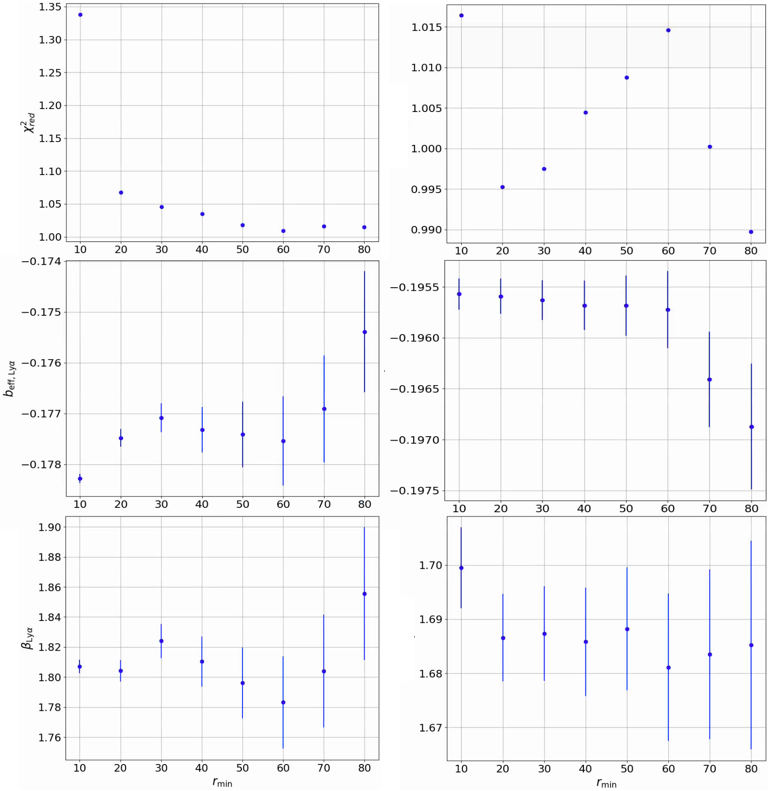
\includegraphics[scale=0.6]{chi2_vs_rmin}
  \caption{Evolution de $\chi_{red}^2$ (ligne du haut), $b_{\mathrm{eff},\mathrm{Ly}\alpha}$ (ligne du milieu) et $\beta_{\mathrm{Ly}\alpha}$ (ligne du bas) en fonction de $r_{\mathrm{min}}$ (donné en \si{\perh\Mpc}). La colonne de gauche donne les mesures avec l'ajustement de la corrélation \lya{}$\times$\lya{} estimée à partir des raw mocks. Celle de droite donne la mesure faite sur les mocks eboss-0.0.}
  \label{fig:chi2_vs_rmin}
\end{figure}

\newpage
\section{Analyse des mocks}
Comme expliqué dans la section~\ref{sec:quickquasars}, nous produisons différentes versions de mocks : les raw mocks, pour lesquels le champ $\delta_F$ est obtenu directement à partir des vraies transmissions, et les mocks après l'utilisation de \texttt{quickquasars} : eboss-0.0, eboss-0.2 et eboss-0.3.
Nous présentons dans cette section l'analyse de ces différentes versions de mocks.
% Pour chacune des versions, nous calculons les fonctions de corrélation \lya{}$\times$\lya{} et \lya{}$\times$QSO. 

\subsection{Analyse des raw mocks}
% Nous présentons premièrement l'analyse des raw mocks.
% Pour les cents réalisations produites, nous avons calculé l'auto corrélation et la corrélation croisée des raw mocks.
Pour chacune des \Nmocks{} réalisations produites, nous avons estimé les fonctions de corrélation \lya{}$\times$\lya{} et \lya{}$\times$QSO des raw mocks.
L'analyse de ces fonctions de corrélation permet d'identifier plus facilement les problèmes qui peuvent exister au niveau de la construction des mocks, car les effets dus à l'ajustement du continuum et les effets astrophysiques et instrumentaux introduits par \texttt{quickquasars} ne sont pas présents. Nous commençons donc par valider la construction des mocks, via l'étude des raw mocks, puis nous présentons l'analyse des versions des mocks avec quickquasars.

Les fonctions de corrélation présentées ici sont estimées dans quatre bins en redshift. Ces bins sont les mêmes que ceux choisis pour analyser les données et déterminer $b_{\mathrm{Ly}\alpha}(z)$ et $\beta_{\mathrm{Ly}\alpha}(z)$ à utiliser pour la construction des mocks (voir chapitre~\ref{prov}). Ces bins sont : $[\num{0}\,;\num{2.35}]$, $[\num{2.35}\,;\num{2.65}]$, $[\num{2.65}\,;\num{3.05}]$ et $[\num{3.05}\,;\num{10}]$. Nous utilisons les mêmes bins afin de faciliter la comparaison entre les mocks et les données.
Une fois les fonctions de corrélation estimées dans chaque bin et pour chaque réalisation, nous calculons, dans chaque bin en redshift, la moyenne de ces fonctions de corrélation, puis ajustons le résultat de cette moyenne. L'ajustement est fait avec le code \texttt{picca}.

\subsubsection{L'auto-corrélation \lya{}$\times$\lya{}}
La figure~\ref{fig:cf_ebossraw_4bins} donne la moyenne des \Nmocks{} fonctions de corrélation \lya{}$\times$\lya{} des raw mocks dans chaque bin en redshift.
Pour chaque bin en redshift, la fonction de corrélation est présentée dans quatre bins en $\mu$ différents. Le bin $\num{0.95} < \mu < 1$ correspond aux paires avec une séparation le long de la ligne de visée. Le bin $\num{0} < \mu < \num{0.5}$ correspond aux paires perpendiculaires à la ligne de visée.
Les lignes continues donnent le meilleur ajustement du modèle produit par \texttt{picca}.
% Nous pouvons remarquer que les raw mocks sont en excellent accord avec le modèle de \texttt{picca}.
Ce modèle décrit très bien les raw mocks.
\textbf{Les lignes en pointillés donnent la prédiction des mocks. L'écart visible entre la corrélation estimée à partir des raw mocks et la prédiction provient de l'écart entre la corrélation du champ $\delta_g$ et la prédiction que nous en faisons (voir figure~\ref{fig:xi_g}). Cet écart se propage lorsque nous passons de la prédiction de $\xi_g$ à la prédiction de $\xi_F$ grâce à l'équation~\ref{eq:xig2xif}.}
% \begin{figure}
%   \centering
%   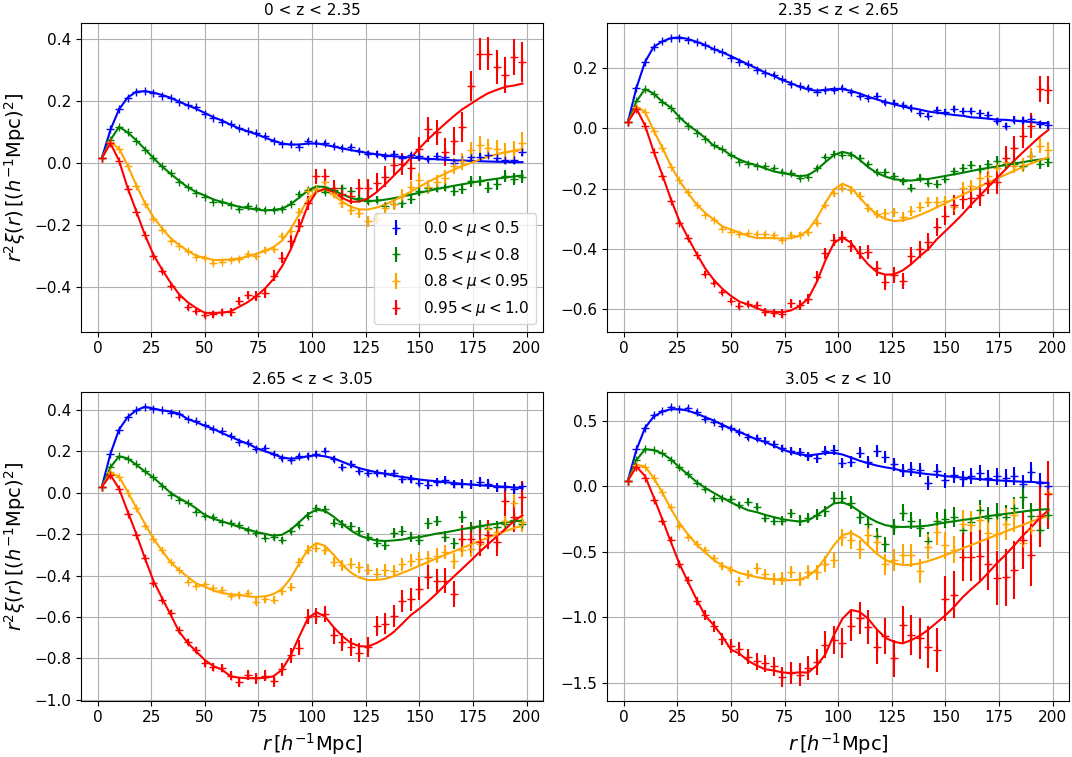
\includegraphics[scale=0.4]{cf_eboss00_4bins}
%   \caption{L'auto-corrélation \lya{}$\times$\lya{} calculée sur les raw mocks. Chaque graphique donne la moyenne des fonctions de corrélation calculées dans chaque bins en redshift pour chaque réalisation. Les fonctions de corrélation sont présentées dans quatre bins en $\mu$. Les lignes continues donnent le meilleur ajustement du modèle produit par \texttt{picca}.}
%   \label{fig:cf_eboss00_4bins}
% \end{figure}
\begin{figure}
  \centering
  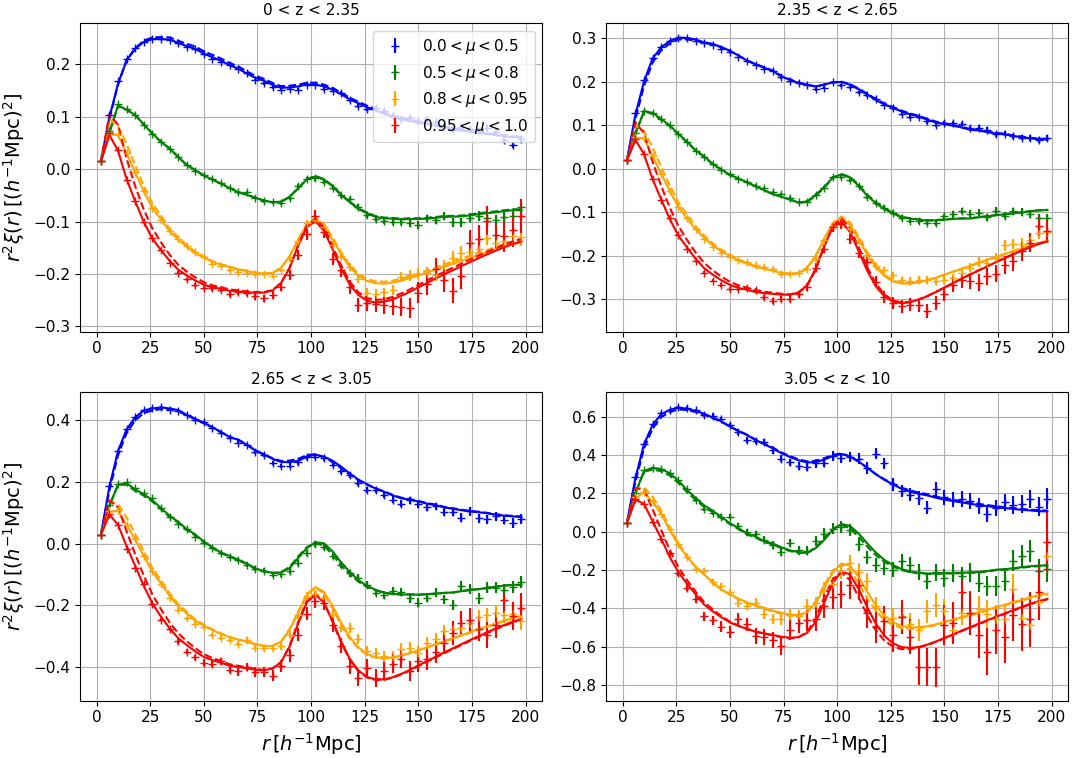
\includegraphics[scale=0.4]{cf_ebossraw_4bins_pred}
  \caption{L'auto-corrélation \lya{}$\times$\lya{} calculée sur la moyenne des \Nmocks{} raw mocks. Chaque graphique donne la moyenne des fonctions de corrélation calculées dans chaque bins en redshift pour chaque réalisation. Les fonctions de corrélation sont présentées dans quatre bins en $\mu$. Les lignes continues donnent le meilleur ajustement du modèle. Les lignes en pointillés donnent la prédiction des mocks.}
  \label{fig:cf_ebossraw_4bins}
\end{figure}

\begin{table}[]
  \centering
  \caption{Résultats de l'ajustement de l'auto-corrélation \lya{}$\times$\lya{} calculée sur la moyenne des \Nmocks{} raw mocks. Chaque colonne donne le résultat de l'ajustement d'un bin en redshift. La première section du tableau donne les paramètres du modèle qui sont ajustés. La seconde donne le redshift effectif $z_{\mathrm{eff}}$ et le $\chi^2$. Le nombre de bins sur lesquels le modèle est ajusté est $N_{bin} = \num{1574}$, ce qui donne un nombre de degrés de liberté $n_{d.o.f.} = \num{1570}$. La dernière section donne le biais et le biais effectif du \lya{}.}
  \label{tab:cf_ebossraw_4bins}
  \begin{tabular}{lcccc}
\toprule
Param\`etre  & $\num{0} < z < \num{2.35}$ & $\num{2.35} < z < \num{2.65}$ & $\num{2.65} < z < \num{3.05}$ & $\num{3.05} < z < \num{10}$ \\
\midrule
$\apar{} $ & $ 1.001 \pm 0.005$ & $ 1.004 \pm 0.004$ & $ 0.998 \pm 0.005$ & $ 0.986 \pm 0.014$ \\
$\aperp{} $ & $ 0.999 \pm 0.007$ & $ 1.002 \pm 0.006$ & $ 0.984 \pm 0.008$ & $ 0.994 \pm 0.018$ \\
$b_{\eta, \mathrm{Ly}\alpha} $ & $ -0.1751 \pm 0.0004$ & $ -0.1936 \pm 0.0004$ & $ -0.2311 \pm 0.0008$ & $ -0.2692 \pm 0.0019$ \\
$\beta_{\mathrm{Ly}\alpha} $ & $ 2.085 \pm 0.014$ & $ 1.863 \pm 0.011$ & $ 1.494 \pm 0.011$ & $ 1.2 \pm 0.016$ \\
\midrule
$\chi^2$ & $ 1557 $ & $ 1608 $ & $ 1628 $ & $ 1534 $ \\
$z_{\mathrm{eff}}$ & $ 2.101 $ & $ 2.237 $ & $ 2.542 $ & $ 2.866 $ \\
\midrule
$b_{\mathrm{Ly}\alpha} $ & $ -0.0808 \pm 0.0004$ & $ -0.1004 \pm 0.0004$ & $ -0.1507 \pm 0.0007$ & $ -0.2198 \pm 0.0017$ \\
$b_{\mathrm{eff}, \mathrm{Ly}\alpha} $ & $ -0.1458 \pm 0.0002$ & $ -0.1721 \pm 0.0002$ & $ -0.2355 \pm 0.0004$ & $ -0.3176 \pm 0.0011$ \\
\bottomrule
  \end{tabular}
\end{table}

\begin{figure}
  \centering
  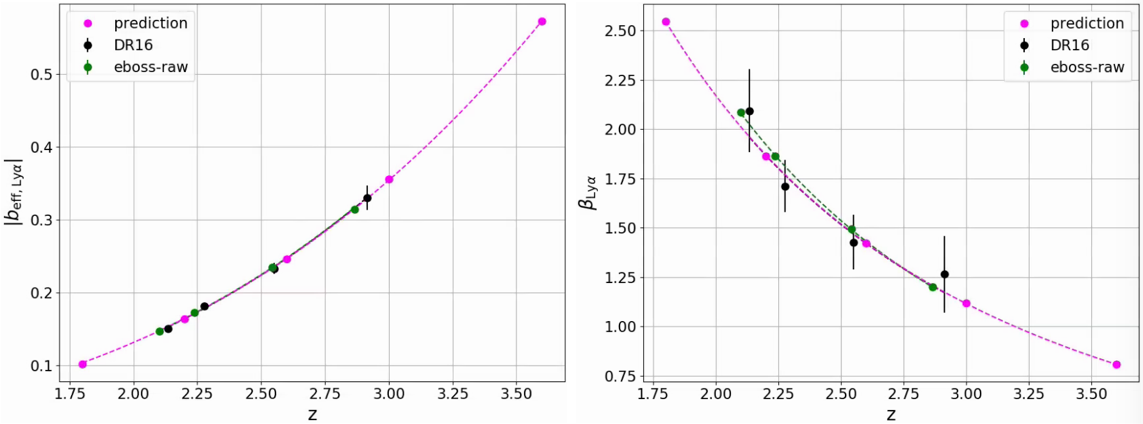
\includegraphics[scale=0.4]{bias_pred}
  \caption{Mesures des paramètres $b_{\mathrm{Ly}\alpha}$ et $\beta_{\mathrm{Ly}\alpha}$ faites avec les auto-corrélations \lya{}$\times$\lya{} estimées dans chaque bin en redshift à partir des données DR16 (noir) et de la moyenne des \Nmocks raw mocks (vert). Les barres d'erreur sont affichées pour ces deux jeux de données. Dans le cas des raw mocks, elles sont plus petites que la taille des points. Les points magenta donnent les mesures faites avec la prédiction des mocks. Les lignes en pointillés représentent l'ajustement sur chaque jeu de données d'une loi de puissance $(1+z)^{\gamma}$.}
  \label{fig:bias_pred}
\end{figure}
% \paragraph{}
% \#prov Est-ce qu'il faut pas que le paragraphe qui suit soit pour l'ajustement combiné de la CF et XCF ?
% Sachant que le biais et beta lya sont déterminés sur le fit en 4 bins de la CF des données, c'est peut-être mieux de faire uniquement sur la CF. Je peux ensuite présenter l'évolution du biais des QSO en fitant la XCF, avec les parametres lya fixés à ce que je trouve dans le fit de la CF ? Ou alors je fais le fit combiné, mais dans ce cas là si une partie du lya passe dans les QSO (ou inversement), j'aurais pas le bon biais QSO.

% Nous présentons maintenant le résultat de l'analyse en quatre bins en redshift des raw mocks. Pour chacune des réalisations, les fonctions de corrélation ont été calculées dans quatre bins en redshift distincts. Une fois toutes ces fonctions de corrélation produites, nous avons calculé la moyenne des cent fonctions de corrélation dans chacun des quatres bins en redshift. Puis, nous avons ajustés ces quatre fonctions de corrélation séparément avec \texttt{picca}.

Le tableau~\ref{tab:cf_ebossraw_4bins} donne le résultat de l'ajustement dans chaque bin en redshift.
Nous pouvons remarquer que les paramètres BAO $\apar{}$ et $\aperp{}$ sont compatibles avec 1.
La figure~\ref{fig:bias_pred} présente le biais et le paramètre RSD du \lya{} obtenus dans l'ajustement des fonctions de corrélation \lya{}$\times$\lya{} des raw mocks (vert), ainsi que ceux obtenus dans l'ajustement des données (noir). 
L'analyse en quatre bins en redshift des données est décrite dans la section~\ref{prov}.
Les valeurs obtenues avec la prédiction lors de l'ajustement des paramètres des mocks sont indiquées en magenta.
% Pour chaque bin en redshift, nous générons la prédiction au redshift effectif du bin. Les biais et paramètres RSD mesurés sur la prédiction sont présentés en (couleur).
Enfin, pour chacun des jeux des données présentés sur la figure~\ref{fig:bias_pred}, nous ajustons une loi de puissance du type $a (1+z)^{\gamma}$.
Les paramètres $b_{\mathrm{Ly}\alpha}$ et $\beta_{\mathrm{Ly}\alpha}$ mesurés sur les raw mocks sont en très bon accord avec ceux prédits, et donc, par construction, avec les données DR16.
Nous pouvons cependant noter une légère déviation entre $\beta_{\mathrm{Ly}\alpha}$ mesuré dans les raw mocks et la valeur prédite pour les faibles redshifts.
% Ceci peut être dû à la forme de la distribution du nombre de paires en fonction du redshift qui peut modifier le paramètre $c$ évalué au redshift effectif de la mesure.
\textbf{Ceci peut être dû à la forme de la distribution du nombre de paires de pixels en fonction du redshift : la prédiction est générée avec un $c(z)$ constant, évalué au redshift $z$ pour lequel la prédiction est calculée, alors que dans le cas des raw mocks, $c(z)$ est évalué au redshift $z$ de chaque pixel. La distribution du nombre de paires en fonction du redshift, dont les variations sont importantes aux faibles redshifts, pourrait impacter le paramètre $c$ effectif pour ces redshifts.}



\subsubsection{La corrélation croisée \lya{}$\times$QSO}

\#prov probleme avec les xcf
% Nous présentons maintenant la même analyse que précédemment, mais en considérant cette fois ci les cent fonctions de corrélation croisée \lya{}$\times$QSO calculées sur les raw mocks. La figure~\ref{prov} (\#prov faire la figure) présente la moyenne de ces cent fonctions de corrélation croisées. La fonction de corrélation est montrée dans quatre bins en redshift. La ligne continue (couleur) donne l'ajustement du modèle produit par \texttt{picca}. La prédiction est montrée en (couleur).
% \#prov conclusion


% \paragraph{}
% Comme précédemment, nous présentons l'analyse en quatre bins en redshift.
% Le tableau~\ref{prov} (\#prov faire le tableau) donne le résultat de l'ajustement dans chaque bin en redshift. Pour cet ajustement, nous avons fixé les paramètres \lya{} à ce que nous avons obtenu dans la section précédente. Ceci nous permet d'obtenir une mesure des paramètres des quasars moins corrélée avec la mesure des paramètres \lya{}. (\#prov donner les correlations de bLya et betaLya avec les autres paramètres ?).
% La figure~\ref{prov} (\#prov faire la figure) montre le biais et le paramètres RSD des quasars obtenus avec un tel ajustement.
% La ligne en pointillés donne le biais $b_{\textsc{QSO}}$ utilisé pour construire le champ des quasars (voir section~\ref{subsec:qso}).
% \#prov conclusion



\subsubsection{Le spectre de puissance à une dimension}

\#prov montrer le P1D des raw mocks ? Plutot celui obtenu avec quickquasars ?
oui, mais probleme pour l'instant.
Montrer quand meme les plots, dire qu'on comprend pas d'ou ca vient, mais montrer que lors de la procedure d'ajustement on obtient les bons P1D?


\subsubsection{La corrélation à une dimension \lya{}$\times$\lya{}}
Contrairement aux autres fonctions de corrélation, la corrélation à une dimension \lya{}$\times$\lya{} n'est pas estimée dans différents bins en redshift. Nous l'estimons sur une seule réalisation des raw mocks, en considérant les forêts de l'ensemble des quasars.
La figure~\ref{fig:cf1d_ebossraw} présente cette corrélation.
Du fait qu'elle est estimée à partir des raw mocks, elle ne possède ni les distorsions produites par l'ajustement du continuum, ni les HCD et les métaux. Nous ne comparons donc pas cette corrélation à celle des données. Cette comparaison est faite en utilisant la corrélation à une dimension estimée à partir des mocks eboss-0.3, présentée sur la figure~\ref{prov}.
% A titre indicatif, la corrélation à une dimension estimée à partir des données DR16 est aussi représentée.
% Les deux corrélations affichées sont normalisées par $\xi^{\mathrm{1D}}(0)$, c'est à dire la variance de $\delta_F$.
% Il serait maladroit de comparer ces deux fonctions de corrélation, car celle estimée à partir des raw mocks ne possède ni les distorsions produites par l'ajustement du continuum, ni les HCD et les métaux. 
% Pour obtenir une comparaison correcte de la fonction de corrélation à une dimension des mocks et des données, nous compararons la corrélation estimées à partir des mocks eboss-0.3 (voir figure~\ref{prov}).

\begin{figure}
  \centering
  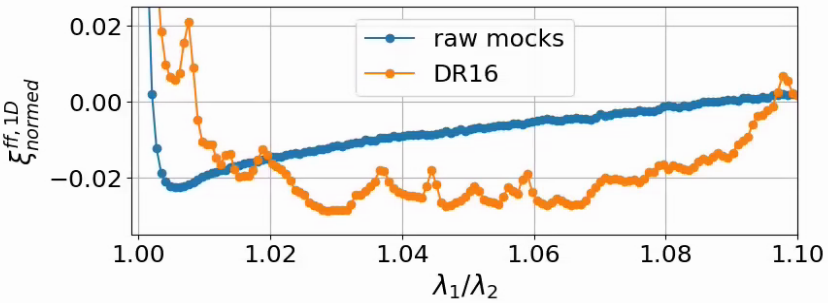
\includegraphics[scale=0.5]{cf1d_ebossraw}
  \caption{La fonction de corrélation à une dimension \lya{}$\times$\lya{} estimée à partir d'une réalisation de raw mocks (bleu).}
  \label{fig:cf1d_ebossraw}
\end{figure}


\subsubsection{L'auto-corrélation QSO$\times$QSO}
\label{subsubsec:auto_qso}
Nous présentons ici la mesure de l'auto-corrélation QSO$\times$QSO, estimée grâce à l'équation~\ref{eq:estimateur_co}.
Comme pour les corrélations \lya{}$\times$\lya{} et \lya{}$\times$QSO, la fonction de corrélation QSO$\times$QSO est estimée puis ajustée dans les quatre bins en redshift $[\num{0}\,;\num{2.35}]$, $[\num{2.35}\,;\num{2.65}]$, $[\num{2.65}\,;\num{3.05}]$ et $[\num{3.05}\,;\num{10}]$.
La corrélation est estimée à partir de 10 réalisations.
% Pour chacun de ces bins, nous estimons la corrélation de dix réalisations des raw mocks, puis nous calculons et ajustons la moyenne de ces dix fonctions de corrélation.
% La figure~\ref{fig:auto_qso_4bins} présente la moyenne des dix fonctions de corrélation et leur modèle ajusté dans chaque bin en redshift.
La figure~\ref{fig:auto_qso_4bins} présente la moyenne des dix fonctions de corrélation et son ajustement dans chaque bin en redshift.
Pour chacun des bins, la fonction de corrélation est présentée dans trois bins en $\mu$. 

\begin{figure}
  \centering
  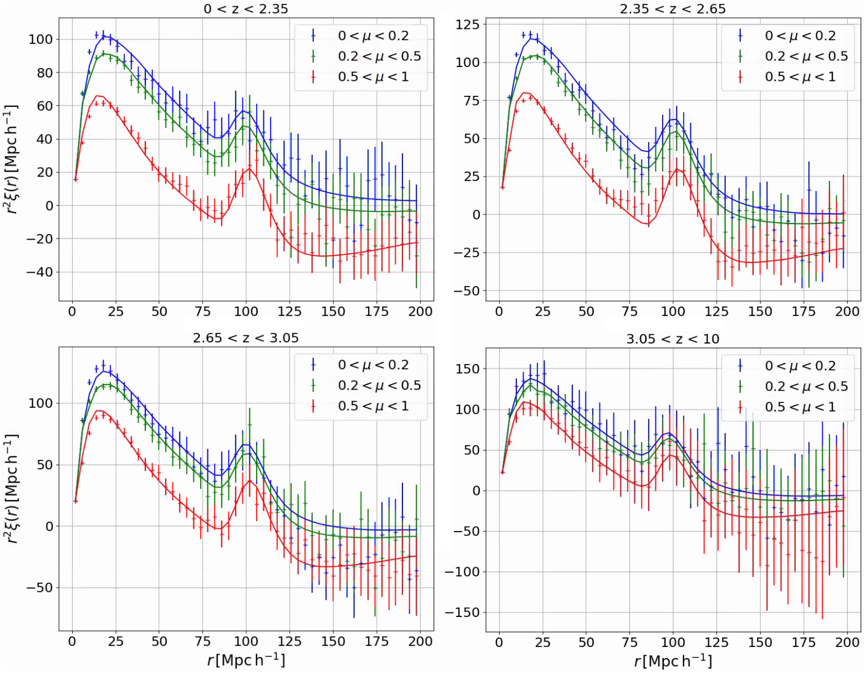
\includegraphics[scale=0.4]{auto_qso_4bins}
  \caption{L'auto-corrélation QSO$\times$QSO calculée sur 10 réalisations des mocks. Chaque graphique donne la moyenne des dix fonctions de corrélation calculées dans chaque bin en redshift. Les fonctions de corrélation sont présentées dans trois bins en $\mu$. Les lignes continues donnent le meilleur ajustement du modèle.}
  \label{fig:auto_qso_4bins}
\end{figure}

\textbf{Le modèle utilisé pour ajuster la corrélation QSO$\times$QSO est le même que celui utilisé pour ajuster la corrélation \lya{}$\times$\lya{}, à la différence que nous n'incluons pas le terme représentant le lissage gaussien. % Le biais et le paramètre RSD ajustés donnent les paramètres des quasars. Ils sont représentés sur la figure~\ref{prov}.
Nous n'incluons pas non plus le terme représentant l'effet produit par la taille non nulle des voxels, mais il serait justifié de le faire.
Dans le cas de la corrélation QSO$\times$QSO, contrairement au cas du \lya{}, nous avons la relation $b_{\textsc{QSO}} \beta_{\textsc{QSO}} = f$, où $f$ est le taux de croissance des structures.
% Lors de l'ajustement, nous fixons donc le paramètre $b_{\eta, \textsc{QSO}} = 1$, et nous ajustons les paramètres $\beta_{\textsc{QSO}}$ et $f$. Les résultats de l'ajustement dans chaque bin en redshift est donné dans le tableau~\ref{tab:auto_qso_4bins}.
Ainsi, plutôt que d'ajuster le paramètre $b_{\eta} = b \beta / f$ comme dans le cas du \lya{} (voir équation~\ref{eq:def_bias}), nous fixons le paramètre $b_{\eta, \textsc{QSO}} = 1$ et nous ajustons les paramètres $\beta_{\textsc{QSO}}$ et $f$.
Le résultat de l'ajustement dans chaque bin en redshift est donné dans le tableau~\ref{tab:auto_qso_4bins}.
Nous pouvons voir dans ce tableau que les paramètres $\apar{}$ et $\aperp{}$ sont compatibles avec 1 à moins de $2 \sigma $.}

\begin{table}[]
  \centering
  \caption{Résultats de l'ajustement de l'auto-corrélation QSO$\times$QSO. Chaque colonne donne le résultat de l'ajustement d'un bin en redshift. La première section du tableau donne les paramètres du modèle qui sont ajustés. La seconde donne le redshift effectif $z_{\mathrm{eff}}$  et le $\chi^2$. Le nombre de bins sur lesquels le modèle est ajusté est $N_{bin} = \num{1574}$, ce qui donne un nombre de degrés de liberté $n_{d.o.f.} = \num{1570}$. La dernière section donne le biais des quasars.}
  \label{tab:auto_qso_4bins}
  \begin{tabular}{lcccc}
    \toprule
    Param\`etre  & $\num{0} < z < \num{2.35}$ & $\num{2.35} < z < \num{2.65}$ & $\num{2.65} < z < \num{3.05}$ & $\num{3.05} < z < \num{10}$ \\
    \midrule
    $\apar{} $ & $ 0.986 \pm 0.019$ & $ 0.97 \pm 0.016$ & $ 0.978 \pm 0.018$ & $ 1.002 \pm 0.045$ \\
    $\aperp{} $ & $ 1.022 \pm 0.012$ & $ 1.01 \pm 0.009$ & $ 1.015 \pm 0.01$ & $ 1.045 \pm 0.024$ \\
    $\beta_{\mathrm{QSO}} $ & $ 0.314 \pm 0.009$ & $ 0.254 \pm 0.007$ & $ 0.204 \pm 0.008$ & $ 0.18 \pm 0.02$ \\
    $f$ & $ 0.99 \pm 0.02$ & $ 1.01 \pm 0.02$ & $ 0.96 \pm 0.03$ & $ 1.01 \pm 0.1$ \\
    \midrule
    $\chi^2$ & $ 1739 $ & $ 1612 $ & $ 1561 $ & $ 1021 $ \\
    $z_{\mathrm{eff}}$ & $ 2.05 $ & $ 2.488 $ & $ 2.826 $ & $ 3.257 $ \\
    \midrule
    $b_{\mathrm{QSO}} $ & $ 3.134 \pm 0.02$ & $ 3.968 \pm 0.02$ & $ 4.71 \pm 0.03$ & $ 5.617 \pm 0.094$ \\
    \bottomrule
  \end{tabular}
\end{table}
\begin{figure}
  \centering
  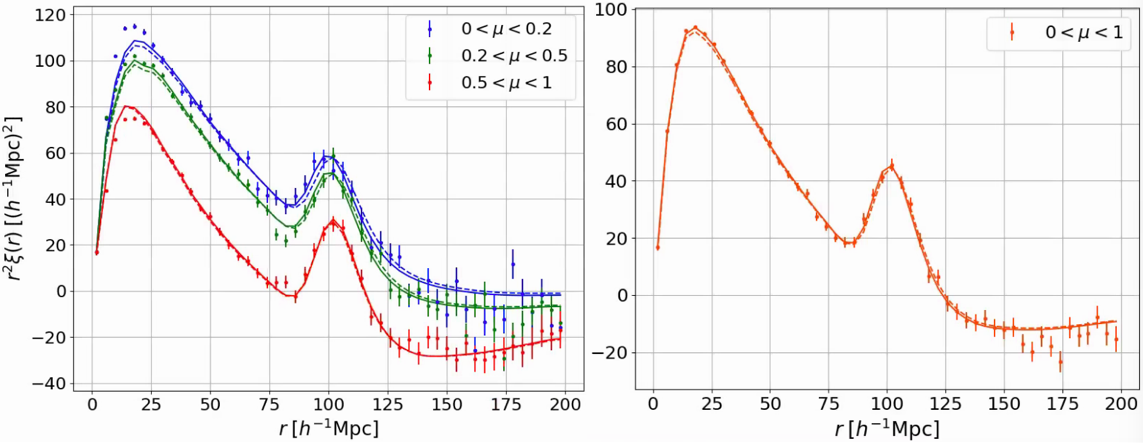
\includegraphics[scale=0.4]{auto_qso}
  \caption{L'auto-corrélation QSO$\times$QSO calculée sur 10 réalisations des mocks et moyennée sur les quatres bins en redshift. Le graphique de gauche présente la corrélation dans trois bins en $\mu$. Celui de droite présente la corrélation moyennée sur toute la gamme en $\mu$. Les lignes continues donnent le meilleur ajustement du modèle. Les lignes en pointillés donnent la prédiction.}
  \label{fig:auto_qso}
\end{figure}

\textbf{Sur la figure~\ref{fig:auto_qso_4bins}, nous pouvons remarquer que le modèle ajusté par picca décrit très bien les mocks. Une légère différence est visible à petit $r$. Cette différence dépend de $\mu$ : l'amplitude est trop faible le long de la ligne de visée, et trop importante perpendiculairement à cette dernière. Ceci semble provenir des RSD aux petites échelles.
Le graphique de droite de la figure~\ref{fig:auto_qso} confirme cette hypothèse : la corrélation moyennée sur toute la gamme en $\mu$ est très bien décrite par le modèle de \texttt{picca} (ligne continue) ainsi que par la prédiction de cette corrélation (ligne en pointillés).}

Enfin, la figure~\ref{fig:bias_auto_qso} présente $b_{\textsc{QSO}}$ et $\beta_{\textsc{QSO}}$ obtenus avec l'ajustement de la moyenne des dix fonctions de corrélation.
La ligne bleue donne la paramétrisation utilisée dans les mocks (équation~\ref{eq:b_qso}).
les valeurs ajustées de $\beta_{\textsc{QSO}}$ et $f$ sont corrélées à plus de \SI{99}{\percent}. Ceci vient du fait que, pour les quasars, le paramètre RSD est faible. Il y a donc peu de différences entre la corrélation le long de la ligne de visée et perpendiculairement à cette dernière.
Malgré cette corrélation, les valeurs obtenues pour $b_{\textsc{QSO}}$ et $\beta_{\textsc{QSO}}$ sont en très bon accord avec la paramétrisation utilisée pour construire les mocks.
% Malgré le fait que $\beta_{\textsc{QSO}}$ et $f$ sont corrélés à plus de \SI{99}{\percent}
% Pour les petits redshifts, $b_{\textsc{QSO}}$ est trop faible et $\beta_{\textsc{QSO}}$ est trop grand grand.
% Cependant, les valeurs ajustées de $\beta_{\textsc{QSO}}$ et $f$ sont corrélées à plus de \SI{99}{\percent}. Ceci vient du fait que, pour les quasars, le paramètre RSD est faible. Il y a donc peu de différences entre la corrélation le long de la ligne de visée et perpendiculairement à cette dernière.
% Lorsque nous fixons $f$ à ce qui est donné par la cosmologie utilisée (équation~\ref{eq:par_cosmo}), nous obtenons un biais et un paramètre RSD en très bon accord avec la paramétrisation utilisée. La figure~\ref{fig:bias_auto_qso_fixed_f} montre $b_{\textsc{QSO}}$ et $\beta_{\textsc{QSO}}$ obtenus avec un tel ajustement.
\begin{figure}
  \centering
  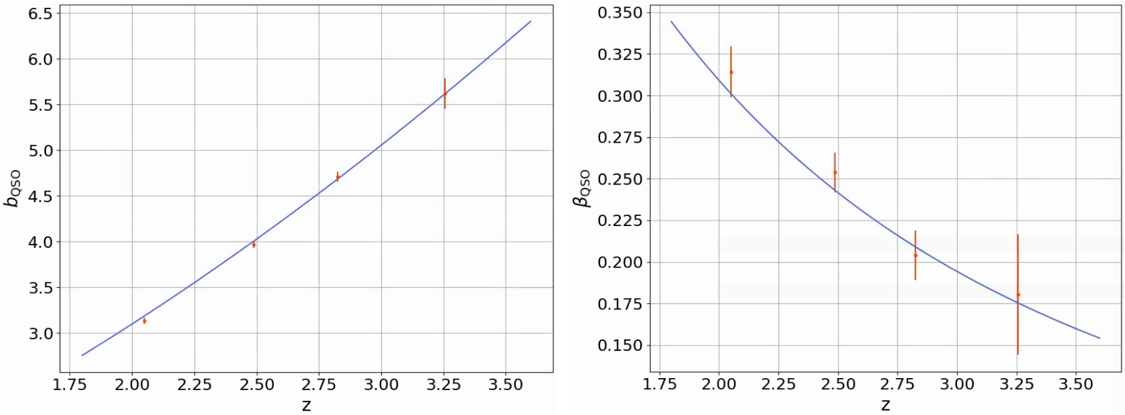
\includegraphics[scale=0.42]{bias_auto_qso}
  \caption{Le biais $b_{\textsc{QSO}}$ et le paramètre RSD $\beta_{\textsc{QSO}}$ mesurés sur l'auto-corrélation QSO$\times$QSO dans les mocks. La mesure est faite dans 4 bins en redshift. La ligne bleue correspond à la paramétrisation utilisée pour construire le relevé de quasars dans les mocks.}
  \label{fig:bias_auto_qso}
\end{figure}
% \begin{figure}
%   \centering
%   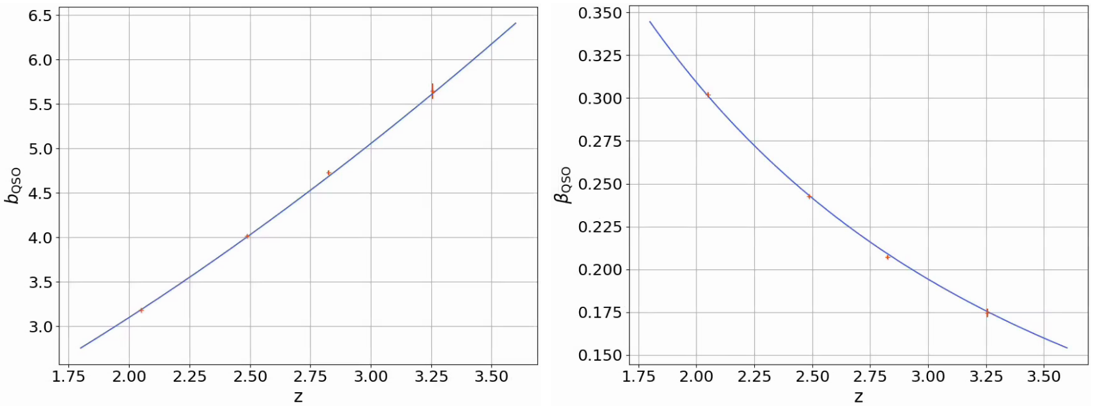
\includegraphics[scale=0.4]{bias_auto_qso_fixed_f}
%   \caption{bla}
%   \label{fig:bias_auto_qso_fixed_f}
% \end{figure}

% La mesure de $b_{\textsc{QSO}}$ et $\beta_{\textsc{QSO}}$ est montrée sur la figure~\ref{prov}.

\subsubsection{L'auto-corrélation HCD$\times$HCD}

Similairement à l'auto-corrélation QSO$\times$QSO, nous estimons la corrélation HCD$\times$HCD. Cependant, celle-ci est produite dans un unique bin en redshift. Nous estimons la corrélation HCD$\times$HCD sur dix réalisations, puis nous calculons et ajustons la moyenne de ces dix corrélations.
La figure~\ref{fig:auto_hcd} présente cette fonction de corrélation. Les lignes continues donnent le modèle ajusté par \texttt{picca}.
La modélisation utilisée pour cette corrélation est la même que celle utilisée pour les quasars. Les deux paramètres ajustés sont donc $f$ et $\beta_{\textsc{HCD}}$.
Le tableau~\ref{tab:auto_hcd} donne le résultat de l'ajustement.
\textbf{Le biais des HCD que nous mesurons est $b_{\mathrm{HCD}} = \num{2.045} \pm \num{0.016}$.
Cette mesure n'est pas compatible avec le biais $b_{\mathrm{HCD}} = 2$ que nous utilisons pour tirer les HCD. 
Cet écart provient très probablement d'une estimation pas assez précise de $\sigma_l$, utilisé dans le calcul du seuil $\nu$ auquel nous avons recours pour tirer les HCD (voir section~\ref{subsec:hcd}).}

\begin{figure}
  \centering
  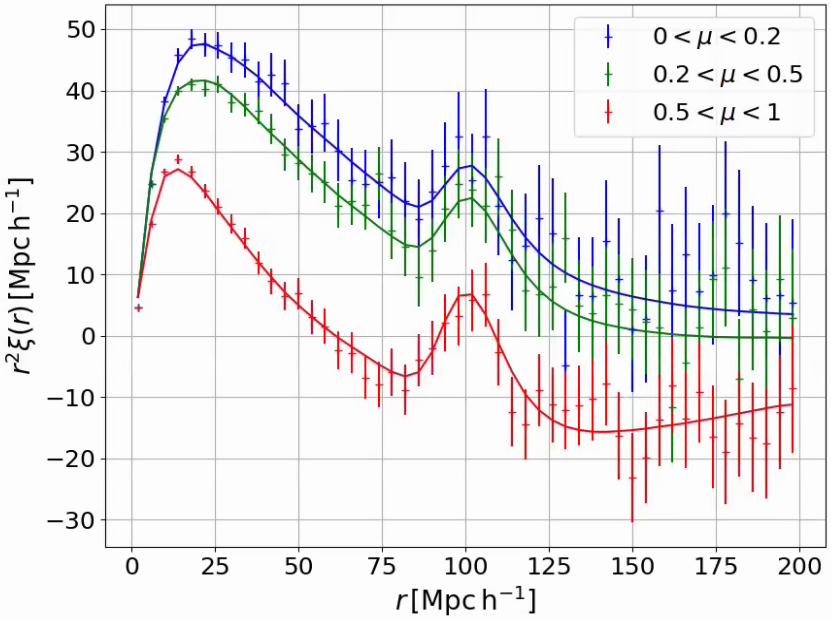
\includegraphics[scale=0.42]{auto_hcd}
  \caption{L'auto-corrélation HCD$\times$HCD calculée sur les mocks. La fonction de corrélation sont présentée dans trois bins en $\mu$. Les lignes continues donnent le meilleur ajustement du modèle dans chaque bin en $\mu$.}
  \label{fig:auto_hcd}
\end{figure}


\begin{table}[]
  \centering
  \caption{Résultats de l'ajustement de l'auto-corrélation HCD$\times$HCD calculée sur les mocks. La première section du tableau donne les paramètres du modèle qui sont ajustés. La seconde donne le redshift effectif $z_{\mathrm{eff}}$ et le $\chi^2$. Le nombre de bins sur lesquels le modèle est ajusté est $N_{bin} = \num{1574}$, ce qui donne un nombre de degrés de liberté $n_{d.o.f.} = \num{1570}$. La dernière section donne le biais des HCD.}
  \label{tab:auto_hcd}
  \begin{tabular}{lc}
    \toprule
    Param\`etre  & $\num{0} < z < \num{10}$ \\
    \midrule
    $\apar{} $ & $ 1.019 \pm 0.02$ \\
    $\aperp{} $ & $ 1.005 \pm 0.014$ \\
    $\beta_{\mathrm{HCD}} $ & $ 0.491 \pm 0.012$ \\
    $f$ & $ 1.0 \pm 0.02$ \\
    \midrule
    $\chi^2$ & $ 1802 $ \\
    $z_{\mathrm{eff}}$ & $ 2.22 $ \\
    \midrule
    $b_{\mathrm{HCD}} $ & $ 2.045 \pm 0.016$ \\
\bottomrule
  \end{tabular}
\end{table}

\newpage
\subsection{Analyse des mocks eboss-0.0}
Maintenant que nous avons vérifié que les raw mocks possèdent les bonnes fonctions de corrélation, nous pouvons analyser les mocks après avoir appliqué \texttt{quickquasars}.
Nous commençons par présenter l'analyse des mocks eboss-0.0.
% Afin de calculer le champ $\delta_F$, nous avons recours à l'ajustement du continuum. Les modèles incluent donc la matrice de distorsion. Contrairement aux raw mocks, les mocks issus de \texttt{quickquasars} contiennent du bruit instrumental. Les fonctions de corrélation sont donc plus bruitées.
Contrairement aux raw mocks, nous avons recours à l'ajustement du continuum pour calculer le champ $\delta_F$. Ainsi, les fonctions de corrélation possèdent les distorsions liées à cet ajustement, et les modèles sont multipliés par les matrices de distorsions (équation~\ref{eq:model_dist}). De plus, les mocks issus de \texttt{quickquasars} contiennent du bruit instrumental. Les fonctions de corrélation sont donc plus bruitées que celles calculées sur les raw mocks.
De la même manière que pour les raw mocks, les fonctions de corrélation sont estimées dans les bins en redshift : $[\num{0}\,;\num{2.35}]$, $[\num{2.35}\,;\num{2.65}]$, $[\num{2.65}\,;\num{3.05}]$ et $[\num{3.05}\,;\num{10}]$. Ces fonctions de corrélation sont calculées sur \Nmocks{} réalisations.


\subsubsection{L'auto-corrélation \lya{}$\times$\lya{}}
% \#prov figure du stack des CF dans les 4 bins en mu + modèle picca lya only ou prédiction * dmat \\
% + tableau qui donne le résultat du fit ? \\
% + figure qui montre l'évolution avec z du biais et beta ? Le plot de la section précédente + le b et beta obtenu pour eboss-0.0 ; ou alors je fais un seul plot avec toutes les versions : raw mocks, eboss-0.0, eboss-0.2, eboss-0.3, prediction, data
La figure~\ref{fig:cf_eboss00_4bins} présente l'auto-corrélation \lya{}$\times$\lya{} calculée sur les mocks eboss-0.0. Chacun des graphiques donne la corrélation dans un des bins en redshift. Pour chaque bins en redshift, la corrélation est présentée dans quatre bins en $\mu$.
% L'auto-corrélation \lya{}$\times$\lya{} estimée sur les mocks eboss-0.0 est en très bon accord avec le modèle ajusté par \texttt{picca}.
Le modèle ajusté par \texttt{picca} décrit très bien l'auto-corrélation \lya{}$\times$\lya{} estimée sur les mocks eboss-0.0.
Le meilleur ajustement du modèle est représenté par des lignes continues. Le résultat des ajustements est donné dans le tableau~\ref{tab:cf_eboss00_4bins}. Comme dans le cas des raw mocks, les paramètres $\apar{}$ et $\aperp{}$ sont compatibles avec 1.

La figure~\ref{fig:bias_cf} présente les paramètres $b_{\mathrm{Ly}\alpha}$ et $\beta_{\mathrm{Ly}\alpha}$ mesurés dans l'auto-corrélation \lya{}$\times$\lya{} estimée à partir des mocks eboss-0.0. Nous pouvons noter un écart statistiquement significatif entre les paramètres \lya{} mesurés sur les raw mocks (vert) et sur les mocks eboss-0.0 (bleu). Cet écart est probablement dû à la matrice de distorsion qui ne capture pas l'intégralité des effets produits par l'ajustement du continuum.

\begin{figure}
  \centering
  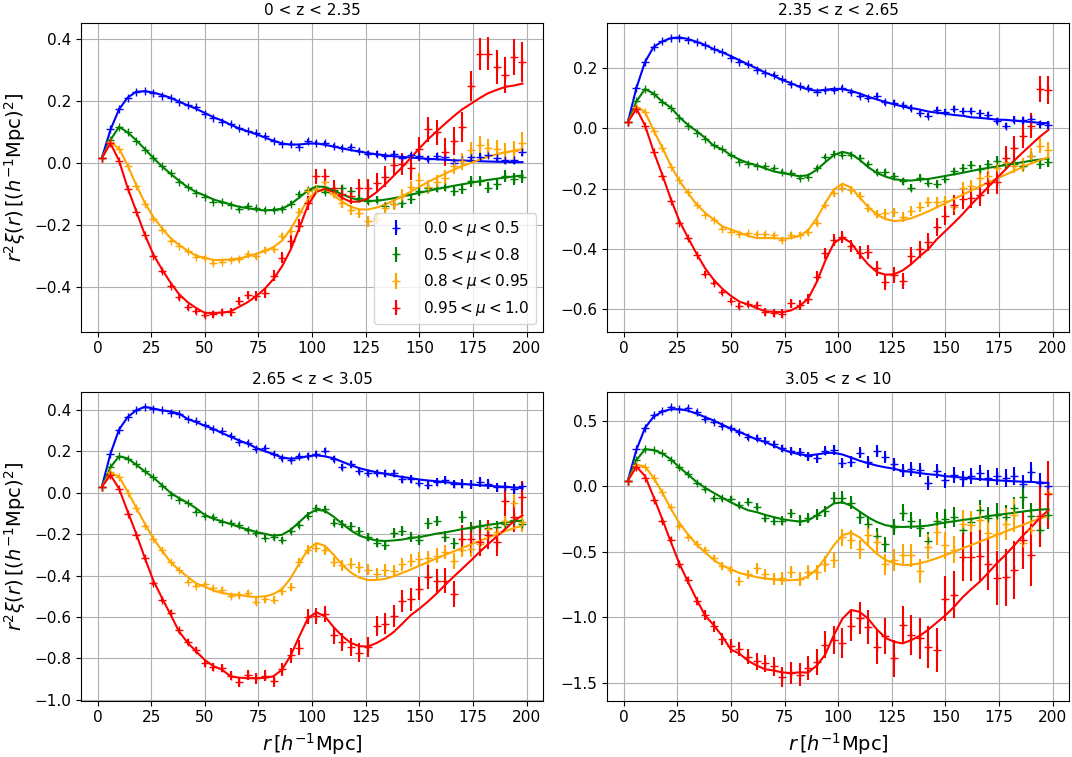
\includegraphics[scale=0.4]{cf_eboss00_4bins}
  \caption{L'auto-corrélation \lya{}$\times$\lya{} calculée sur les mocks eboss-0.0. Chaque graphique donne la moyenne des fonctions de corrélation calculées dans chaque bins en redshift. Les fonctions de corrélation sont présentées dans quatre bins en $\mu$. Les lignes continues donnent le meilleur ajustement du modèle.}
  \label{fig:cf_eboss00_4bins}
\end{figure}

\begin{table}[]
  \centering
  \caption{Résultats de l'ajustement de l'auto-corrélation \lya{}$\times$\lya{} calculée sur les mocks eboss-0.0. Chaque colonne donne le résultat de l'ajustement d'un bin en redshift. La première section du tableau donne les paramètres du modèle qui sont ajustés. La seconde donne le $\chi^2$ et le redshift effectif $z_{\mathrm{eff}}$. Le nombre de bins sur lesquels le modèle est ajusté est $N_{bin} = \num{1574}$, ce qui donne un nombre de degrés de liberté $n_{d.o.f.} = \num{1570}$. La dernière section donne le biais et le biais effectif du \lya{}.}
  \label{tab:cf_eboss00_4bins}
  \begin{tabular}{lcccc}
    \toprule
    Param\`etre  & $\num{0} < z < \num{2.35}$ & $\num{2.35} < z < \num{2.65}$ & $\num{2.65} < z < \num{3.05}$ & $\num{3.05} < z < \num{10}$ \\
    \midrule
    $\apar{} $ & $ 0.992 \pm 0.009$ & $ 1.006 \pm 0.007$ & $ 1.005 \pm 0.009$ & $ 0.954 \pm 0.023$ \\
    $\aperp{} $ & $ 1.002 \pm 0.016$ & $ 1.0 \pm 0.012$ & $ 0.981 \pm 0.013$ & $ 1.057 \pm 0.033$ \\
    $b_{\eta, \mathrm{Ly}\alpha} $ & $ -0.1868 \pm 0.0007$ & $ -0.2045 \pm 0.0007$ & $ -0.2381 \pm 0.0012$ & $ -0.2752 \pm 0.0029$ \\
    $\beta_{\mathrm{Ly}\alpha} $ & $ 1.962 \pm 0.016$ & $ 1.768 \pm 0.012$ & $ 1.454 \pm 0.013$ & $ 1.172 \pm 0.02$ \\
    \midrule
    $\chi^2$ & $ 1498 $ & $ 1622 $ & $ 1598 $ & $ 1629 $ \\
    $z_{\mathrm{eff}}$ & $ 2.118 $ & $ 2.254 $ & $ 2.54 $ & $ 2.867 $ \\
    \midrule
    $b_{\mathrm{Ly}\alpha} $ & $ -0.0916 \pm 0.0004$ & $ -0.1118 \pm 0.0004$ & $ -0.1595 \pm 0.0007$ & $ -0.23 \pm 0.0018$ \\
    $b_{\mathrm{eff}, \mathrm{Ly}\alpha} $ & $ -0.1607 \pm 0.0002$ & $ -0.1873 \pm 0.0002$ & $ -0.2467 \pm 0.0004$ & $ -0.3298 \pm 0.0011$ \\
    \bottomrule
  \end{tabular}
\end{table}



\subsubsection{La corrélation croisée \lya{}$\times$QSO}
La figure~\ref{fig:xcf_eboss00_4bins} présente la corrélation croisée \lya{}$\times$QSO dans chaque bin de redshift.
Contrairement à l'auto-corrélation \lya{}$\times$\lya{}, la corrélation \lya{}$\times$QSO est estimée pour $\rpar{} \in [-200;\;200] \si{\perh\Mpc}$.
Ainsi, pour obtenir chaque bin en $\mu$, nous moyennons la fonction de corrélation pour les valeurs positives et négatives de $\mu$.
% Dans chacun des bins en redshift, la corrélation est ajustée dans la gamme $r \in [20;\;180] \si{\perh\Mpc}$, ce qui correspond à un nombre de bins en $(\rpar{}, \rperp{})$ $N_{bin} = \num{3148}$, soit le double du nombre de bins utilisés pour ajuster l'auto-corrélation \lya{}$\times$\lya{}.
Comme pour les autres corrélations, la corrélation \lya{}$\times$QSO est ajustée dans la gamme $r \in [20;\;180] \si{\perh\Mpc}$, ce qui correspond à un nombre de bins en $(\rpar{}, \rperp{})$ $N_{bin} = \num{3148}$, soit le double du nombre de bins utilisés pour ajuster l'auto-corrélation \lya{}$\times$\lya{}.

\textbf{Comme expliqué dans la section~\ref{subsec:model_donnees}, à cause de la dégénérescence entre les paramètres du \lya{} et ceux des quasars, nous fixons les paramètres $b_{\textsc{QSO}}$ et $\beta_{\textsc{QSO}}$. Ces paramètres sont fixés à la valeur donnée par la paramétrisation (équation~\ref{eq:b_qso}) évaluée au redshift effectif de chaque ajustement. Ceci est validé par la mesure de $b_{\textsc{QSO}}$ et $\beta_{\textsc{QSO}}$ avec l'auto-corrélation QSO$\times$QSO, qui est en accord avec la paramétrisation utilisée (voir section~\ref{subsubsec:auto_qso}).
Nous pouvons remarquer sur la figure~\ref{fig:xcf_eboss00_4bins} que, comme pour l'auto-corrélation \lya$\times$\lya{}, le modèle ajusté par picca décrit très bien la corrélation croisée \lya{}$\times$QSO.}
% Comme pour l'auto-corrélation, la corrélation croisée \lya{}$\times$QSO est en très bon accord avec le modèle ajusté par \texttt{picca}.

Le tableau~\ref{tab:xcf_eboss00_4bins} présente le résultat de l'ajustement dans chaque bin de redshift.
Nous pouvons noter que le paramètre $\Delta_{\rpar{}, \textsc{QSO}}$ est compatible avec 0, ce à quoi nous nous attendons. Une légère tension ($\num{2.3}\sigma$) est visible pour le bin $\num{2.65} < z < \num{3.05}$, nous attribuons cela à une fluctuation statistique.
\textbf{Aussi, comme dans le cas de l'auto-corrélation, les paramètres $\apar{}$ et $\aperp{}$ sont compatibles avec 1.
Cependant, les paramètres du \lya{} mesurés dans la corrélation croisée sont en tension avec ceux mesurés dans l'auto-corrélation \lya{}$\times$\lya{}. Pourtant, du fait que les paramètres des quasars mesurés sur la corrélation QSO$\times$QSO sont en accord avec la paramétrisation du biais des quasars utilisée dans les mocks, nous nous attendons à mesurer les mêmes $b_{\mathrm{Ly}\alpha}$ et $\beta_{\mathrm{Ly}\alpha}$ dans l'auto-corrélation \lya{}$\times$\lya{} et dans la corrélation croisée \lya{}$\times$QSO.
Nous avons essayé de fixer $\Delta_{\rpar{}, \textsc{QSO}} = 0$ dans les ajustements des corrélations croisées. Nous avons aussi essayé de réduire $r_{\mathrm{min}}$ à \SI{10}{\perh\Mpc} dans l'ajustement des corrélations \lya{}$\times$\lya{} et \lya{}$\times$QSO.
Mais ces essais ne réduisent pas les tensions observés.}

\begin{figure}
  \centering
  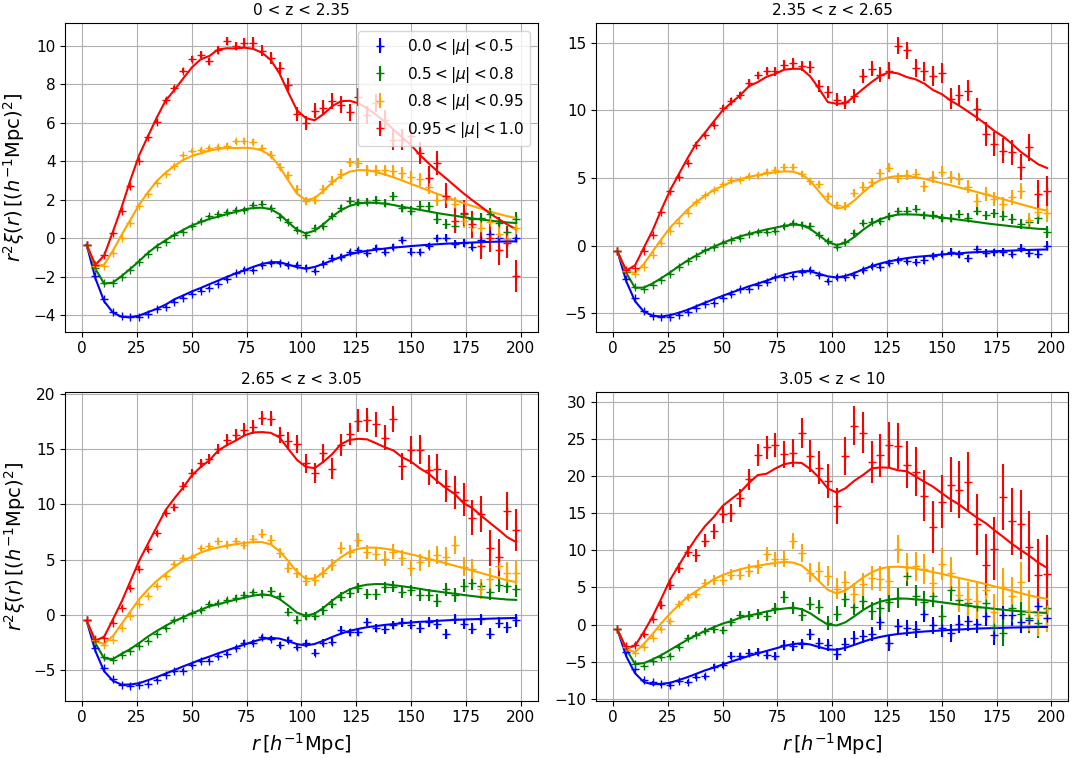
\includegraphics[scale=0.4]{xcf_eboss00_4bins}
  \caption{La corrélation croisée \lya{}$\times$QSO calculée sur les mocks eboss-0.0. Chaque graphique donne la moyenne des fonctions de corrélation calculées dans chaque bins en redshift. Les fonctions de corrélation sont présentées dans quatre bins en $\mu$. Les lignes continues donnent le meilleur ajustement du modèle.}
  \label{fig:xcf_eboss00_4bins}
\end{figure}

\begin{table}[]
  \centering
  \caption{Résultats de l'ajustement de la corrélation croisée \lya{}$\times$QSO calculée sur les mocks eboss-0.0. Chaque colonne donne le résultat de l'ajustement d'un bin en redshift. La première section du tableau donne les paramètres du modèle qui sont ajustés. La seconde donne le $\chi^2$ et le redshift effectif $z_{\mathrm{eff}}$. Le nombre de bins sur lesquels le modèle est ajusté est $N_{bin} = \num{3148}$, ce qui donne un nombre de degrés de liberté $n_{d.o.f.} = \num{3143}$. La dernière section donne le biais et le biais effectif du \lya{}.}
  \label{tab:xcf_eboss00_4bins}
  \begin{tabular}{lcccc}
% \toprule
% Param\`etre  & $\num{0} < z < \num{2.35}$ & $\num{2.35} < z < \num{2.65}$ & $\num{2.65} < z < \num{3.05}$ & $\num{3.05} < z < \num{10}$ \\
% \midrule
% $\apar{} $ & $ 1.002 \pm 0.008$ & $ 0.99 \pm 0.008$ & $ 0.984 \pm 0.012$ & $ 1.008 \pm 0.026$ \\
% $\aperp{} $ & $ 1.003 \pm 0.01$ & $ 1.002 \pm 0.01$ & $ 0.988 \pm 0.013$ & $ 1.024 \pm 0.032$ \\
% $b_{\eta, \mathrm{Ly}\alpha} $ & $ -0.1723 \pm 0.0013$ & $ -0.1991 \pm 0.0017$ & $ -0.2296 \pm 0.003$ & $ -0.2963 \pm 0.0088$ \\
% $\beta_{\mathrm{Ly}\alpha} $ & $ 1.823 \pm 0.027$ & $ 1.59 \pm 0.025$ & $ 1.234 \pm 0.026$ & $ 1.275 \pm 0.062$ \\
% $\Delta_{\rpar{}, \textsc{QSO}}$ & $ -0.0492 \pm 0.053$ & $ 0.0401 \pm 0.0588$ & $ -0.1877 \pm 0.082$ & $ 0.2434 \pm 0.1982$ \\
% \midrule
% $\chi^2$ & $ 3424 $ & $ 3520 $ & $ 6441 $ & $ 3826 $ \\
% $z_{\mathrm{eff}}$ & $ 2.128 $ & $ 2.362 $ & $ 2.663 $ & $ 3.043 $ \\
% \midrule
% $b_{\mathrm{Ly}\alpha} $ & $ -0.091 \pm 0.0008$ & $ -0.1215 \pm 0.001$ & $ -0.1816 \pm 0.0019$ & $ -0.2283 \pm 0.0054$ \\
% $b_{\mathrm{eff}, \mathrm{Ly}\alpha} $ & $ -0.1544 \pm 0.0005$ & $ -0.1946 \pm 0.0007$ & $ -0.2649 \pm 0.0012$ & $ -0.3367 \pm 0.0036$ \\
% % $b_{\mathrm{QSO}} $ & $ 3.326 \pm 0.0$ & $ 3.761 \pm 0.0$ & $ 4.352 \pm 0.0$ & $ 5.145 \pm 0.0$ \\
% \bottomrule
\toprule
Param\`etre  & $\num{0} < z < \num{2.35}$ & $\num{2.35} < z < \num{2.65}$ & $\num{2.65} < z < \num{3.05}$ & $\num{3.05} < z < \num{10}$ \\
\midrule
$\apar{} $ & $ 1.002 \pm 0.008$ & $ 0.99 \pm 0.008$ & $ 0.986 \pm 0.012$ & $ 1.005 \pm 0.026$ \\
$\aperp{} $ & $ 1.0 \pm 0.01$ & $ 1.001 \pm 0.01$ & $ 1.001 \pm 0.013$ & $ 1.013 \pm 0.031$ \\
$b_{\eta, \mathrm{Ly}\alpha} $ & $ -0.1717 \pm 0.0013$ & $ -0.1985 \pm 0.0017$ & $ -0.2333 \pm 0.003$ & $ -0.294 \pm 0.0088$ \\
$\beta_{\mathrm{Ly}\alpha} $ & $ 1.787 \pm 0.027$ & $ 1.564 \pm 0.024$ & $ 1.344 \pm 0.029$ & $ 1.208 \pm 0.058$ \\
$\Delta_{\rpar{}, \textsc{QSO}}$ & $ -0.051 \pm 0.0527$ & $ 0.0393 \pm 0.0585$ & $ -0.1822 \pm 0.0854$ & $ 0.2128 \pm 0.1919$ \\
\midrule
$\chi^2$ & $ 3233 $ & $ 3410 $ & $ 3238 $ & $ 3410 $ \\
$z_{\mathrm{eff}}$ & $ 2.128 $ & $ 2.362 $ & $ 2.663 $ & $ 3.043 $ \\
\midrule
$b_{\mathrm{Ly}\alpha} $ & $ -0.0925 \pm 0.0008$ & $ -0.1231 \pm 0.001$ & $ -0.1696 \pm 0.0018$ & $ -0.239 \pm 0.0054$ \\
$b_{\mathrm{eff}, \mathrm{Ly}\alpha} $ & $ -0.1556 \pm 0.0005$ & $ -0.1959 \pm 0.0007$ & $ -0.2548 \pm 0.0012$ & $ -0.3462 \pm 0.0036$ \\
% $b_{\mathrm{QSO}} $ & $ 3.326 \pm 0.0$ & $ 3.761 \pm 0.0$ & $ 4.352 \pm 0.0$ & $ 5.145 \pm 0.0$ \\
\bottomrule
  \end{tabular}
\end{table}


\newpage
\subsection{Analyse des mocks eboss-0.2}
Nous analysons à présent les mocks eboss-0.2. Ces mocks sont obtenus comme les mocks eboss-0.0, analysés précédemment, à la différence que le code \texttt{quickquasars} inclue les HCD dans les spectres synthétiques.
Comme pour les données, nous masquons les HCD pour lesquels $\log n_{\textsc{HI}} > \num{20.3}$. Cependant, dans le cas des mocks, le masquage s'effectue à partir du vrai catalogue de HCD.
Lors de l'ajustement des fonctions de corrélation, nous modélisons les HCD non masqués.
Nous présentons dans la section~\ref{prov} l'analyse d'une réalisation eboss-0.2 où les DLA ont été masqués en utilisant l'algorithme d'identification utilisé pour les données DR16.


\subsubsection{L'auto-corrélation \lya{}$\times$\lya{}}
La figure~\ref{fig:cf_eboss02_4bins} présente les fonctions d'auto-corrélation \lya{}$\times$\lya{} dans chaque bin en redshift estimées à partir des mocks eboss-0.2. Comme précédemment, les corrélations sont présentées dans quatre bins en $\mu$.
Les lignes continues donnent le meilleur ajustement du modèle produit par \texttt{picca}.
Le tableau~\ref{tab:cf_eboss02_4bins} donne le résultat de l'ajustement dans chaque bin en redshift.
A cause du masquage des DLA, le nombre de paires de pixels utilisées pour estimer la corrélation \lya{}$\times$\lya{} est réduit, ce qui résulte dans une augmentation légère des barres d'erreurs.
Cependant, nous pouvons noter que les $\chi^2$ augmentent légèrement par rapport à l'ajustement de la corrélation \lya{}$\times$\lya{} estimée à partir des mocks eboss-0.0, ce qui suggère que la modélisation des HCD n'est pas parfaite.
\textbf{Le biais des HCD mesuré dans chaque bin en redshift est compatible avec 0.
Nous pensons que ceci est dû à un manque de statistique : lorsque nous ajustons la moyenne pondérée des quatre bins en redshift, nous mesurons $b_{\textsc{HCD}} = \num{-0.0082} \pm \num{0.0008}$.
Par ailleurs, nous n'observons pas de changement significatif dans l'ajustement de cette corrélation lorsque nous l'ajustons avec $r_{\mathrm{min}} = \SI{10}{\perh\Mpc}$.}
% \#prov le biais HCD est compatible avec 0 dans les 4 bins en z ... \\
% En prenant rmin = 10, j'obtiens un biais 2 fois plus grand : -35 +/- 10 contre -15 +/- 15 \\
% Faire juste une remarque que le biais HCD est compatible avec 0 est dire qu'on regarde ca dans le chapitre suivant ?

La figure~\ref{fig:bias_cf} présente les paramètres  $b_{\mathrm{Ly}\alpha}$ et $\beta_{\mathrm{Ly}\alpha}$ mesurés dans l'auto-corrélation \lya{}$\times$\lya{} estimée à partir des mocks eboss-0.2. Nous pouvons remarquer que la mesure de ces paramètres est très affectée par la présence des HCD. Ceci nous laisse croire que la mesure de $b_{\mathrm{Ly}\alpha}$ et $\beta_{\mathrm{Ly}\alpha}$ dans les données DR16, sur laquelle nous avons fondé l'ajustement de nos mocks, n'est pas robuste. Ceci est étudié en détail dans le chapitre suivant.


\begin{figure}
  \centering
  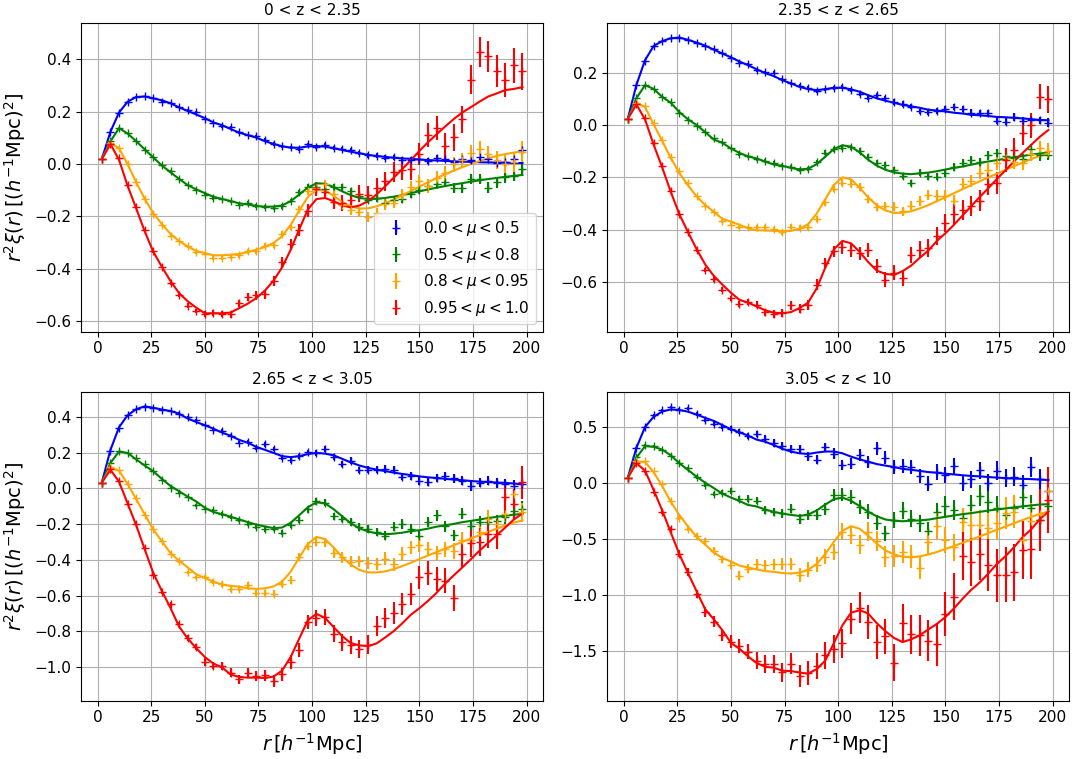
\includegraphics[scale=0.4]{cf_eboss02_4bins}
  \caption{L'auto-corrélation \lya{}$\times$\lya{} calculée sur les mocks eboss-0.2. Chaque graphique donne la moyenne des fonctions de corrélation calculées dans chaque bins en redshift. Les fonctions de corrélation sont présentées dans quatre bins en $\mu$. Les lignes continues donnent le meilleur ajustement du modèle.}
  \label{fig:cf_eboss02_4bins}
\end{figure}

\begin{table}[]
  \centering
  \caption{Résultats de l'ajustement de l'auto-corrélation \lya{}$\times$\lya{} calculée sur les mocks eboss-0.2. Chaque colonne donne le résultat de l'ajustement d'un bin en redshift. La première section du tableau donne les paramètres du modèle qui sont ajustés. La seconde donne le $\chi^2$ et le redshift effectif $z_{\mathrm{eff}}$. Le nombre de bins sur lesquels le modèle est ajusté est $N_{bin} = \num{1574}$, ce qui donne un nombre de degrés de liberté $n_{d.o.f.} = \num{1568}$. La dernière section donne le biais et le biais effectif du \lya{}.}
  \label{tab:cf_eboss02_4bins}
  \begin{tabular}{lcccc}
    \toprule
    Param\`etre  & $\num{0} < z < \num{2.35}$ & $\num{2.35} < z < \num{2.65}$ & $\num{2.65} < z < \num{3.05}$ & $\num{3.05} < z < \num{10}$ \\
    \midrule
    $\apar{} $ & $ 1.005 \pm 0.009$ & $ 0.996 \pm 0.007$ & $ 1.004 \pm 0.009$ & $ 0.936 \pm 0.021$ \\
    $\aperp{} $ & $ 0.985 \pm 0.016$ & $ 1.0 \pm 0.012$ & $ 0.978 \pm 0.013$ & $ 1.066 \pm 0.039$ \\
    $b_{\eta, \mathrm{Ly}\alpha} $ & $ -0.186 \pm 0.0008$ & $ -0.2042 \pm 0.0008$ & $ -0.2365 \pm 0.0014$ & $ -0.2782 \pm 0.0035$ \\
    $\beta_{\mathrm{Ly}\alpha} $ & $ 1.709 \pm 0.023$ & $ 1.568 \pm 0.019$ & $ 1.295 \pm 0.02$ & $ 1.102 \pm 0.032$ \\
    $b_{\textsc{HCD}} $ & $ -0.0015 \pm 0.0015$ & $ -0.0017 \pm 0.0014$ & $ -0.005 \pm 0.0024$ & $ -0.0085 \pm 0.006$ \\
    $\beta_{\textsc{HCD}} $ & $ 0.502 \pm 0.09$ & $ 0.5 \pm 0.09$ & $ 0.501 \pm 0.09$ & $ 0.5 \pm 0.09$ \\
    \midrule
    $\chi^2$ & $ 1535 $ & $ 1579 $ & $ 1627 $ & $ 1650 $ \\
    $z_{\mathrm{eff}}$ & $ 2.117 $ & $ 2.253 $ & $ 2.539 $ & $ 2.866 $ \\
    \midrule
    $b_{\mathrm{Ly}\alpha} $ & $ -0.1048 \pm 0.0012$ & $ -0.1259 \pm 0.0012$ & $ -0.1779 \pm 0.0021$ & $ -0.2474 \pm 0.0053$ \\
    $b_{\mathrm{eff}, \mathrm{Ly}\alpha} $ & $ -0.1729 \pm 0.0011$ & $ -0.2006 \pm 0.001$ & $ -0.2638 \pm 0.0018$ & $ -0.3479 \pm 0.0047$ \\
    \bottomrule
  \end{tabular}
\end{table}

\begin{figure}
  \centering
  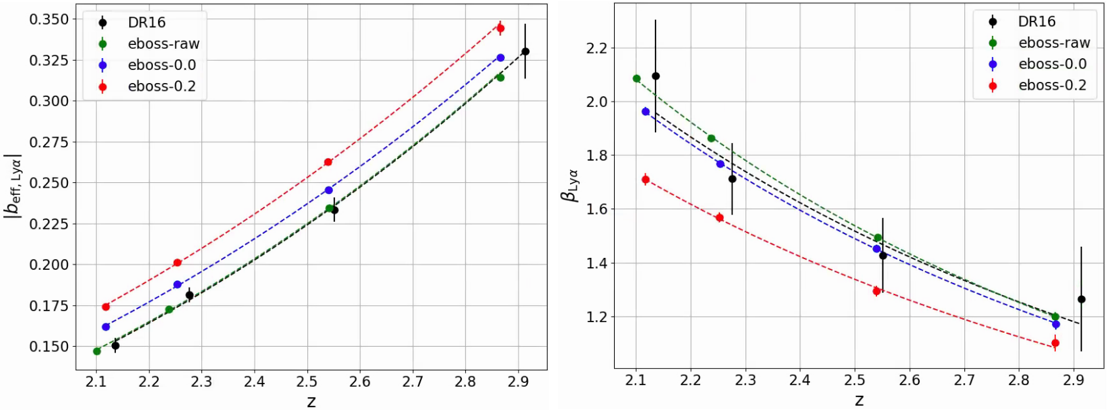
\includegraphics[scale=0.43]{bias_cf}
  \caption{Mesures des paramètres $b_{\mathrm{Ly}\alpha}$ et $\beta_{\mathrm{Ly}\alpha}$ faites avec les auto-corrélations \lya{}$\times$\lya{} estimées dans chaque bin en redshift à partir des données DR16 (noir), des raw mocks (vert), des mocks eboss-0.0 (bleu) et des mocks eboss-0.2 (rouge). Pour chacun de ces jeux de données, les barres d'erreur sont représentées. Cependant, dans le cas des mocks, elles sont souvent plus petites que la taille des points.}
  % L'évolution de $b_{\mathrm{Ly}\alpha}$ et $\beta_{\mathrm{Ly}\alpha}$ en fonction de la version des mocks analysée indique que cette mesure est affectée par les distorsions induites par l'ajustement du continuum, ainsi que par l'ajout des HCD.}
  \label{fig:bias_cf}
\end{figure}


\subsubsection{La corrélation croisée \lya{}$\times$QSO}
La figure~\ref{fig:xcf_eboss02_4bins} présente la mesure de la corrélation croisée \lya{}$\times$QSO. Celle ci est estimée sur \Nmocks{} réalisations eboss-0.2 et dans quatre bins en redshift. Pour chacun des bins en redshift, la fonction de corrélation est présentée dans quatre bins en $\mu$.
Les lignes continues donnent le meilleur ajustement du modèle produit par \texttt{picca}. Il décrit correctement la corrélation estimée dans les mocks.
Le tableau~\ref{tab:xcf_eboss02_4bins} donne le résultat des ajustements dans chaque bin en redshift.
Comme pour les mocks eboss-0.0, la mesure de $\Delta_{\rpar{}, \textsc{QSO}}$ est compatible avec 0.
\textbf{Nous pouvons remarquer dans ce tableau que, comme pour les mocks eboss-0.0, la mesure des paramètres \lya{} dans la corrélation croisée \lya{}$\times$QSO est en tension avec la mesure faite sur l'auto-corrélation \lya{}$\times$\lya{}.
  Aussi, les mesures de $b_{\textsc{HCD}}$ faites sur les corrélations \lya{}$\times$\lya{} et \lya{}$\times$QSO ne sont pas compatibles. Le biais des HCD mesuré dans la corrélation croisée est beaucoup plus important. L'ajustement de la moyenne pondérée des quatre bins en redshift donne $b_{\textsc{HCD}} = -0.0377 \pm 0.0020$, comparé à $b_{\textsc{HCD}} = \num{-0.0082} \pm \num{0.0008}$ mesuré dans l'auto-corrélation.
  Nous pensons que cet écart provient du fait qu'il est difficile lors de l'ajustement du modèle de distinguer l'effet du \lya de celui des HCD. Une partie des HCD est interprétée comme du \lya{}, et vice versa. La proportion de HCD et le \lya{} identifiés dans les corrélations \lya{}$\times$\lya{} et \lya{}$\times$QSO est différente. Ceci est investigué plus en détails dans le chapitre suivant.
  Nous pouvons cependant remarquer que les quantités $b_{\mathrm{Ly}\alpha} + b_{\textsc{HCD}}$ et $b_{\mathrm{Ly}\alpha}\beta_{\mathrm{Ly}\alpha} + b_{\textsc{HCD}}\beta_{\textsc{HCD}}$ (équation~\ref{eq:bias_hcd_def}) mesurés dans les corrélations \lya{}$\times$\lya{} et \lya{}$\times$QSO sont comparables aux données DR16. Ces mesures sont présentées sur la figure~\ref{fig:sum_bias}.
}


\begin{figure}
  \centering
  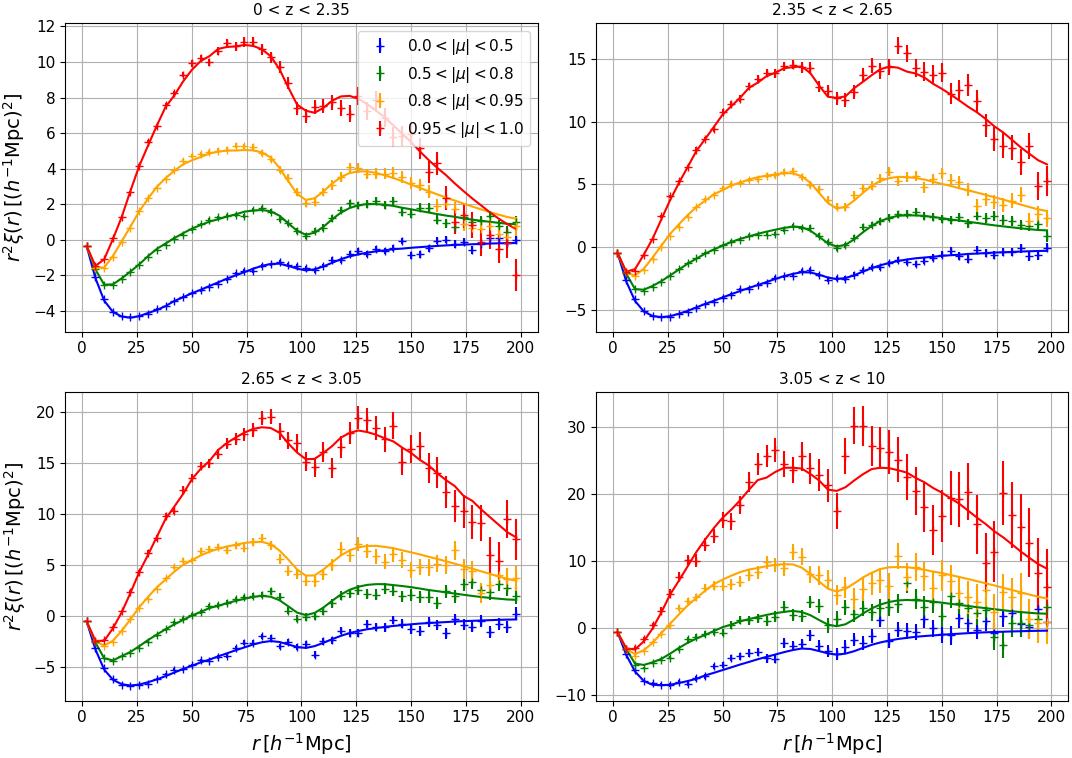
\includegraphics[scale=0.4]{xcf_eboss02_4bins}
  \caption{La corrélation croisée \lya{}$\times$QSO calculée sur les mocks eboss-0.2. Chaque graphique donne la moyenne des fonctions de corrélation calculées dans chaque bins en redshift. Les fonctions de corrélation sont présentées dans quatre bins en $\mu$. Les lignes continues donnent le meilleur ajustement du modèle.}
  \label{fig:xcf_eboss02_4bins}
\end{figure}

\begin{table}[]
  \centering
  \caption{Résultats de l'ajustement de la corrélation croisée \lya{}$\times$QSO calculée sur les mocks eboss-0.2. Chaque colonne donne le résultat de l'ajustement d'un bin en redshift. La première section du tableau donne les paramètres du modèle qui sont ajustés. La seconde donne le $\chi^2$ et le redshift effectif $z_{\mathrm{eff}}$. Le nombre de bins sur lesquels le modèle est ajusté est $N_{bin} = \num{3148}$, ce qui donne un nombre de degrés de liberté $n_{d.o.f.} = \num{3141}$. La dernière section donne le biais et le biais effectif du \lya{}.}
  \label{tab:xcf_eboss02_4bins}
  \begin{tabular}{lcccc}
% \toprule
% Param\`etre  & $\num{0} < z < \num{2.35}$ & $\num{2.35} < z < \num{2.65}$ & $\num{2.65} < z < \num{3.05}$ & $\num{3.05} < z < \num{10}$ \\
% \midrule
% $\apar{} $ & $ 1.005 \pm 0.008$ & $ 0.996 \pm 0.009$ & $ 0.983 \pm 0.013$ & $ 1.017 \pm 0.027$ \\
% $\aperp{} $ & $ 0.993 \pm 0.011$ & $ 0.992 \pm 0.01$ & $ 0.998 \pm 0.013$ & $ 1.001 \pm 0.03$ \\
% $b_{\eta, \mathrm{Ly}\alpha} $ & $ -0.1757 \pm 0.0018$ & $ -0.2017 \pm 0.0023$ & $ -0.2347 \pm 0.0036$ & $ -0.3337 \pm 0.0126$ \\
% $\beta_{\mathrm{Ly}\alpha} $ & $ 2.128 \pm 0.07$ & $ 1.744 \pm 0.06$ & $ 1.248 \pm 0.05$ & $ 3.596 \pm 0.707$ \\
% $b_{\textsc{HCD}} $ & $ -0.0291 \pm 0.0027$ & $ -0.0327 \pm 0.0037$ & $ -0.0199 \pm 0.0065$ & $ -0.1851 \pm 0.0193$ \\
% $\beta_{\textsc{HCD}} $ & $ 0.613 \pm 0.084$ & $ 0.561 \pm 0.086$ & $ 0.503 \pm 0.09$ & $ 0.515 \pm 0.086$ \\
% $\Delta_{\rpar{}, \textsc{QSO}}$ & $ -0.0517 \pm 0.0541$ & $ -0.0377 \pm 0.06$ & $ -0.1791 \pm 0.0853$ & $ 0.1909 \pm 0.1957$ \\
% \midrule
% $\chi^2$ & $ 3360 $ & $ 3332 $ & $ 5537 $ & $ 3623 $ \\
% $z_{\mathrm{eff}}$ & $ 2.127 $ & $ 2.362 $ & $ 2.663 $ & $ 3.043 $ \\
% \midrule
% $b_{\mathrm{Ly}\alpha} $ & $ -0.0795 \pm 0.0023$ & $ -0.1122 \pm 0.0032$ & $ -0.1836 \pm 0.0057$ & $ -0.0912 \pm 0.0165$ \\
% $b_{\mathrm{eff}, \mathrm{Ly}\alpha} $ & $ -0.1449 \pm 0.0019$ & $ -0.1867 \pm 0.0027$ & $ -0.2689 \pm 0.0049$ & $ -0.223 \pm 0.0132$ \\
% % $b_{\mathrm{QSO}} $ & $ 3.326 \pm 0.0$ & $ 3.761 \pm 0.0$ & $ 4.351 \pm 0.0$ & $ 5.145 \pm 0.0$ \\
% \bottomrule
\toprule
Param\`etre  & $\num{0} < z < \num{2.35}$ & $\num{2.35} < z < \num{2.65}$ & $\num{2.65} < z < \num{3.05}$ & $\num{3.05} < z < \num{10}$ \\
\midrule
$\apar{} $ & $ 1.004 \pm 0.008$ & $ 0.996 \pm 0.009$ & $ 0.987 \pm 0.013$ & $ 1.013 \pm 0.027$ \\
$\aperp{} $ & $ 0.991 \pm 0.011$ & $ 0.992 \pm 0.01$ & $ 1.005 \pm 0.014$ & $ 0.992 \pm 0.03$ \\
$b_{\eta, \mathrm{Ly}\alpha} $ & $ -0.1751 \pm 0.0017$ & $ -0.2008 \pm 0.0022$ & $ -0.2427 \pm 0.0044$ & $ -0.3277 \pm 0.0116$ \\
$\beta_{\mathrm{Ly}\alpha} $ & $ 1.991 \pm 0.062$ & $ 1.656 \pm 0.054$ & $ 1.775 \pm 0.094$ & $ 2.281 \pm 0.305$ \\
$b_{\textsc{HCD}} $ & $ -0.0244 \pm 0.0027$ & $ -0.0278 \pm 0.0037$ & $ -0.0672 \pm 0.0067$ & $ -0.137 \pm 0.0192$ \\
$\beta_{\textsc{HCD}} $ & $ 0.583 \pm 0.085$ & $ 0.546 \pm 0.087$ & $ 0.54 \pm 0.085$ & $ 0.502 \pm 0.088$ \\
$\Delta_{\rpar{}, \textsc{QSO}}$ & $ -0.0528 \pm 0.0539$ & $ -0.037 \pm 0.0599$ & $ -0.1784 \pm 0.087$ & $ 0.192 \pm 0.1927$ \\
\midrule
$\chi^2$ & $ 3223 $ & $ 3283 $ & $ 3157 $ & $ 3316 $ \\
$z_{\mathrm{eff}}$ & $ 2.127 $ & $ 2.362 $ & $ 2.663 $ & $ 3.043 $ \\
\midrule
$b_{\mathrm{Ly}\alpha} $ & $ -0.0846 \pm 0.0023$ & $ -0.1176 \pm 0.0032$ & $ -0.1335 \pm 0.0058$ & $ -0.1411 \pm 0.0164$ \\
$b_{\mathrm{eff}, \mathrm{Ly}\alpha} $ & $ -0.1495 \pm 0.0019$ & $ -0.1915 \pm 0.0027$ & $ -0.224 \pm 0.0048$ & $ -0.2663 \pm 0.0136$ \\
% $b_{\mathrm{QSO}} $ & $ 3.326 \pm 0.0$ & $ 3.761 \pm 0.0$ & $ 4.351 \pm 0.0$ & $ 5.145 \pm 0.0$ \\
\bottomrule
  \end{tabular}
\end{table}

\begin{figure}
  \centering
  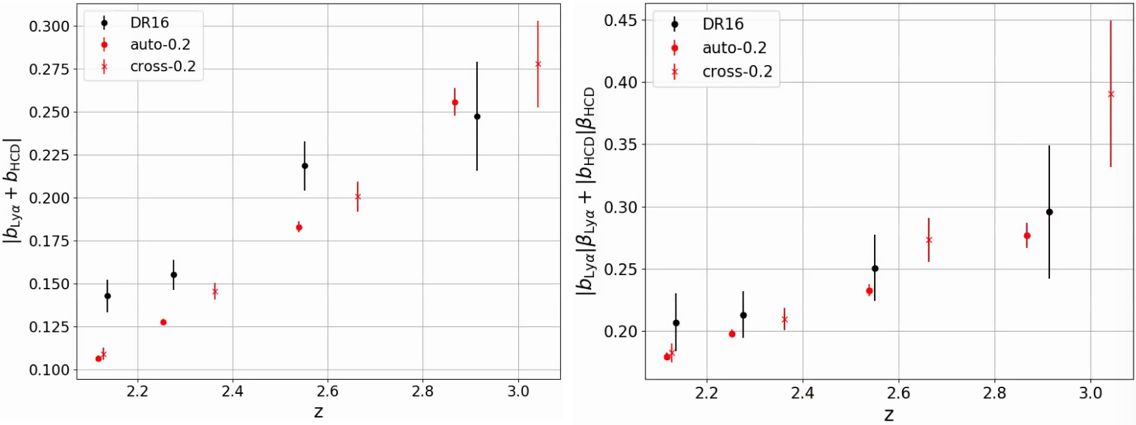
\includegraphics[scale=0.4]{sum_bias}
  \caption{Mesures des paramètres $b_{\mathrm{Ly}\alpha} + b_{\textsc{HCD}}$ et $b_{\mathrm{Ly}\alpha}\beta_{\mathrm{Ly}\alpha} + b_{\textsc{HCD}}\beta_{\textsc{HCD}}$ dans la corrélation \lya{}$\times$\lya{} estimée à partir des données DR16 (noir), dans la corrélations \lya{}$\times$\lya{} estimée à partir des mocks eboss-0.2 (points rouges) et dans la corrélation \lya{}$\times$QSO estimée à partir des mocks eboss-0.2 (croix rouges).}
  \label{fig:sum_bias}
\end{figure}

\newpage
\subsection{Analyse des mocks eboss-0.3}
Cette section présente l'analyse des mocks eboss-0.3. Ces mocks sont obtenus comme les mocks eboss-0.2, analysés précédemment, à la différence que le code \texttt{quickquasars} ajoute les métaux dans les spectres synthétiques. Nous incluons donc les termes $\xi_{m\times n}$ et $\xi_{m\times \textsc{QSO}}$ dans la modélisation des fonctions de corrélation.


\subsubsection{L'auto-corrélation \lya{}$\times$\lya{}}
\#prov figure du stack des CF dans les 4 bins en mu + modele picca lya + hcd + met \\
+ tableau qui donne le résultat du fit ? \\
+ figure qui montre l'évolution avec z du biais et beta ?


\subsubsection{L'auto-corrélation \lya{}$\times$QSO}
\#prov figure du stack des XCF dans les 4 bins en mu. \\
+ tableau qui donne le résultat du fit ? fit avec les parametres lya fixés ?\\ 
+ figure qui montre l'évolution avec z du biais et beta ? 


\subsubsection{Le spectre de puissance à une dimension}
\#prov montrer le P1D ?
Pourquoi pas, pour montrer les metaux ? Ou alors le xi1d

\subsubsection{La fonction de corrélation à une dimension}
Comparer les mocks et les données


% \bibliography{../source/library}
\printbibliography
\end{document}
